% Options for packages loaded elsewhere
% Options for packages loaded elsewhere
\PassOptionsToPackage{unicode}{hyperref}
\PassOptionsToPackage{hyphens}{url}
\PassOptionsToPackage{dvipsnames,svgnames,x11names}{xcolor}
%
\documentclass[
  russian,
  12pt,
  a4paper,
  DIV=11,
  numbers=noendperiod]{scrreprt}
\usepackage{xcolor}
\usepackage{amsmath,amssymb}
\setcounter{secnumdepth}{5}
\usepackage{iftex}
\ifPDFTeX
  \usepackage[T1]{fontenc}
  \usepackage[utf8]{inputenc}
  \usepackage{textcomp} % provide euro and other symbols
\else % if luatex or xetex
  \usepackage{unicode-math} % this also loads fontspec
  \defaultfontfeatures{Scale=MatchLowercase}
  \defaultfontfeatures[\rmfamily]{Ligatures=TeX,Scale=1}
\fi
\usepackage{lmodern}
\ifPDFTeX\else
  % xetex/luatex font selection
  \setmainfont[]{DejaVu Serif}
  \setsansfont[]{DejaVu Sans}
  \setmonofont[]{DejaVu Sans Mono}
\fi
% Use upquote if available, for straight quotes in verbatim environments
\IfFileExists{upquote.sty}{\usepackage{upquote}}{}
\IfFileExists{microtype.sty}{% use microtype if available
  \usepackage[]{microtype}
  \UseMicrotypeSet[protrusion]{basicmath} % disable protrusion for tt fonts
}{}
\usepackage{setspace}
% Make \paragraph and \subparagraph free-standing
\makeatletter
\ifx\paragraph\undefined\else
  \let\oldparagraph\paragraph
  \renewcommand{\paragraph}{
    \@ifstar
      \xxxParagraphStar
      \xxxParagraphNoStar
  }
  \newcommand{\xxxParagraphStar}[1]{\oldparagraph*{#1}\mbox{}}
  \newcommand{\xxxParagraphNoStar}[1]{\oldparagraph{#1}\mbox{}}
\fi
\ifx\subparagraph\undefined\else
  \let\oldsubparagraph\subparagraph
  \renewcommand{\subparagraph}{
    \@ifstar
      \xxxSubParagraphStar
      \xxxSubParagraphNoStar
  }
  \newcommand{\xxxSubParagraphStar}[1]{\oldsubparagraph*{#1}\mbox{}}
  \newcommand{\xxxSubParagraphNoStar}[1]{\oldsubparagraph{#1}\mbox{}}
\fi
\makeatother

\usepackage{color}
\usepackage{fancyvrb}
\newcommand{\VerbBar}{|}
\newcommand{\VERB}{\Verb[commandchars=\\\{\}]}
\DefineVerbatimEnvironment{Highlighting}{Verbatim}{commandchars=\\\{\}}
% Add ',fontsize=\small' for more characters per line
\usepackage{framed}
\definecolor{shadecolor}{RGB}{241,243,245}
\newenvironment{Shaded}{\begin{snugshade}}{\end{snugshade}}
\newcommand{\AlertTok}[1]{\textcolor[rgb]{0.68,0.00,0.00}{#1}}
\newcommand{\AnnotationTok}[1]{\textcolor[rgb]{0.37,0.37,0.37}{#1}}
\newcommand{\AttributeTok}[1]{\textcolor[rgb]{0.40,0.45,0.13}{#1}}
\newcommand{\BaseNTok}[1]{\textcolor[rgb]{0.68,0.00,0.00}{#1}}
\newcommand{\BuiltInTok}[1]{\textcolor[rgb]{0.00,0.23,0.31}{#1}}
\newcommand{\CharTok}[1]{\textcolor[rgb]{0.13,0.47,0.30}{#1}}
\newcommand{\CommentTok}[1]{\textcolor[rgb]{0.37,0.37,0.37}{#1}}
\newcommand{\CommentVarTok}[1]{\textcolor[rgb]{0.37,0.37,0.37}{\textit{#1}}}
\newcommand{\ConstantTok}[1]{\textcolor[rgb]{0.56,0.35,0.01}{#1}}
\newcommand{\ControlFlowTok}[1]{\textcolor[rgb]{0.00,0.23,0.31}{\textbf{#1}}}
\newcommand{\DataTypeTok}[1]{\textcolor[rgb]{0.68,0.00,0.00}{#1}}
\newcommand{\DecValTok}[1]{\textcolor[rgb]{0.68,0.00,0.00}{#1}}
\newcommand{\DocumentationTok}[1]{\textcolor[rgb]{0.37,0.37,0.37}{\textit{#1}}}
\newcommand{\ErrorTok}[1]{\textcolor[rgb]{0.68,0.00,0.00}{#1}}
\newcommand{\ExtensionTok}[1]{\textcolor[rgb]{0.00,0.23,0.31}{#1}}
\newcommand{\FloatTok}[1]{\textcolor[rgb]{0.68,0.00,0.00}{#1}}
\newcommand{\FunctionTok}[1]{\textcolor[rgb]{0.28,0.35,0.67}{#1}}
\newcommand{\ImportTok}[1]{\textcolor[rgb]{0.00,0.46,0.62}{#1}}
\newcommand{\InformationTok}[1]{\textcolor[rgb]{0.37,0.37,0.37}{#1}}
\newcommand{\KeywordTok}[1]{\textcolor[rgb]{0.00,0.23,0.31}{\textbf{#1}}}
\newcommand{\NormalTok}[1]{\textcolor[rgb]{0.00,0.23,0.31}{#1}}
\newcommand{\OperatorTok}[1]{\textcolor[rgb]{0.37,0.37,0.37}{#1}}
\newcommand{\OtherTok}[1]{\textcolor[rgb]{0.00,0.23,0.31}{#1}}
\newcommand{\PreprocessorTok}[1]{\textcolor[rgb]{0.68,0.00,0.00}{#1}}
\newcommand{\RegionMarkerTok}[1]{\textcolor[rgb]{0.00,0.23,0.31}{#1}}
\newcommand{\SpecialCharTok}[1]{\textcolor[rgb]{0.37,0.37,0.37}{#1}}
\newcommand{\SpecialStringTok}[1]{\textcolor[rgb]{0.13,0.47,0.30}{#1}}
\newcommand{\StringTok}[1]{\textcolor[rgb]{0.13,0.47,0.30}{#1}}
\newcommand{\VariableTok}[1]{\textcolor[rgb]{0.07,0.07,0.07}{#1}}
\newcommand{\VerbatimStringTok}[1]{\textcolor[rgb]{0.13,0.47,0.30}{#1}}
\newcommand{\WarningTok}[1]{\textcolor[rgb]{0.37,0.37,0.37}{\textit{#1}}}

\usepackage{longtable,booktabs,array}
\newcounter{none} % for unnumbered tables
\usepackage{calc} % for calculating minipage widths
% Correct order of tables after \paragraph or \subparagraph
\usepackage{etoolbox}
\makeatletter
\patchcmd\longtable{\par}{\if@noskipsec\mbox{}\fi\par}{}{}
\makeatother
% Allow footnotes in longtable head/foot
\IfFileExists{footnotehyper.sty}{\usepackage{footnotehyper}}{\usepackage{footnote}}
\makesavenoteenv{longtable}
\usepackage{graphicx}
\makeatletter
\newsavebox\pandoc@box
\newcommand*\pandocbounded[1]{% scales image to fit in text height/width
  \sbox\pandoc@box{#1}%
  \Gscale@div\@tempa{\textheight}{\dimexpr\ht\pandoc@box+\dp\pandoc@box\relax}%
  \Gscale@div\@tempb{\linewidth}{\wd\pandoc@box}%
  \ifdim\@tempb\p@<\@tempa\p@\let\@tempa\@tempb\fi% select the smaller of both
  \ifdim\@tempa\p@<\p@\scalebox{\@tempa}{\usebox\pandoc@box}%
  \else\usebox{\pandoc@box}%
  \fi%
}
% Set default figure placement to htbp
\def\fps@figure{htbp}
\makeatother



\ifLuaTeX
\usepackage[bidi=basic,shorthands=off,provide=*]{babel}
\else
\usepackage[bidi=default,shorthands=off,provide=*]{babel}
\fi
\ifPDFTeX
\else
\babelfont{rm}[]{DejaVu Serif}
\fi
\ifLuaTeX
  \usepackage{selnolig} % disable illegal ligatures
\fi


\setlength{\emergencystretch}{3em} % prevent overfull lines

\providecommand{\tightlist}{%
  \setlength{\itemsep}{0pt}\setlength{\parskip}{0pt}}



 


\usepackage{juliamono}
\KOMAoption{captions}{tableheading}
\makeatletter
\@ifpackageloaded{caption}{}{\usepackage{caption}}
\AtBeginDocument{%
\ifdefined\contentsname
  \renewcommand*\contentsname{Содержание}
\else
  \newcommand\contentsname{Содержание}
\fi
\ifdefined\listfigurename
  \renewcommand*\listfigurename{Список Иллюстраций}
\else
  \newcommand\listfigurename{Список Иллюстраций}
\fi
\ifdefined\listtablename
  \renewcommand*\listtablename{Список Таблиц}
\else
  \newcommand\listtablename{Список Таблиц}
\fi
\ifdefined\figurename
  \renewcommand*\figurename{Рисунок}
\else
  \newcommand\figurename{Рисунок}
\fi
\ifdefined\tablename
  \renewcommand*\tablename{Таблица}
\else
  \newcommand\tablename{Таблица}
\fi
}
\@ifpackageloaded{float}{}{\usepackage{float}}
\floatstyle{ruled}
\@ifundefined{c@chapter}{\newfloat{codelisting}{h}{lop}}{\newfloat{codelisting}{h}{lop}[chapter]}
\floatname{codelisting}{Список}
\newcommand*\listoflistings{\listof{codelisting}{Список Каталогов}}
\makeatother
\makeatletter
\makeatother
\makeatletter
\@ifpackageloaded{caption}{}{\usepackage{caption}}
\@ifpackageloaded{subcaption}{}{\usepackage{subcaption}}
\makeatother
\usepackage{bookmark}
\IfFileExists{xurl.sty}{\usepackage{xurl}}{} % add URL line breaks if available
\urlstyle{same}
% fallback for those not using the hyperref driver hyperxmp:
\makeatletter
\@ifundefined{xmpquote}{\newcommand{\xmpquote}[1]{#1}}{}
\makeatother
\hypersetup{
  pdftitle={Отчёт по лабораторной работе №1},
  pdfauthor={Нечаева Кира Андреевна},
  pdflang={ru-RU},
  colorlinks=true,
  linkcolor={blue},
  filecolor={Maroon},
  citecolor={Blue},
  urlcolor={Blue},
  pdfcreator={LaTeX via pandoc}}


\title{Отчёт по лабораторной работе №1}
\usepackage{etoolbox}
\makeatletter
\providecommand{\subtitle}[1]{% add subtitle to \maketitle
  \apptocmd{\@title}{\par {\large #1 \par}}{}{}
}
\makeatother
\subtitle{Дисциплина: Математическое моделирование}
\author{Нечаева Кира Андреевна}
\date{2026-01-01}
\begin{document}
\maketitle

\renewcommand*\contentsname{Содержание}
{
\setcounter{tocdepth}{1}
\tableofcontents
}
\listoffigures
\listoftables

\setstretch{1.5}
\chapter{Цель
работы}\label{ux446ux435ux43bux44c-ux440ux430ux431ux43eux442ux44b}

Целью лабораторной работы является подготовка рабочего пространства для
курса, создание проекта DrWatson, установка необходимых пакетов Julia и
выполнение примера модели экспоненциального роста. Также в работе
требуется преобразовать код в литературный стиль, сгенерировать из него
чистый код, Jupyter notebook и документацию Quarto, а затем выполнить
параметрическое исследование модели.

\chapter{Задание}\label{ux437ux430ux434ux430ux43dux438ux435}

В лабораторной работе требуется:

\begin{enumerate}
\def\labelenumi{\arabic{enumi}.}
\tightlist
\item
  Создать рабочий каталог для всего курса.
\item
  Создать рабочее пространство для программ в рамках лабораторной
  работы.
\item
  Выполнить все задания по тексту лабораторной работы.
\item
  Установить необходимые пакеты.
\item
  Выполнить предложенный код.
\item
  Преобразовать код в литературный стиль.
\item
  Сгенерировать из литературного кода чистый код, Jupyter notebook и
  документацию в формате Quarto.
\item
  Выполнить код из Jupyter notebook.
\item
  Интегрировать документацию в формате Quarto в отчёт.
\item
  Добавить вычисление для набора параметров.
\item
  Сгенерировать производные форматы для параметрического кода.
\item
  Выполнить параметрический код из Jupyter notebook.
\item
  Интегрировать документацию с параметрами в отчёт.
\end{enumerate}

\chapter{Выполнение лабораторной
работы}\label{ux432ux44bux43fux43eux43bux43dux435ux43dux438ux435-ux43bux430ux431ux43eux440ux430ux442ux43eux440ux43dux43eux439-ux440ux430ux431ux43eux442ux44b}

\section{Подготовка среды
работы}\label{ux43fux43eux434ux433ux43eux442ux43eux432ux43aux430-ux441ux440ux435ux434ux44b-ux440ux430ux431ux43eux442ux44b}

Работу я выполняла в Windows с использованием WSL и Ubuntu. После
запуска WSL я перешла в домашний каталог и проверила используемую
операционную систему.

\begin{figure}[H]

{\centering 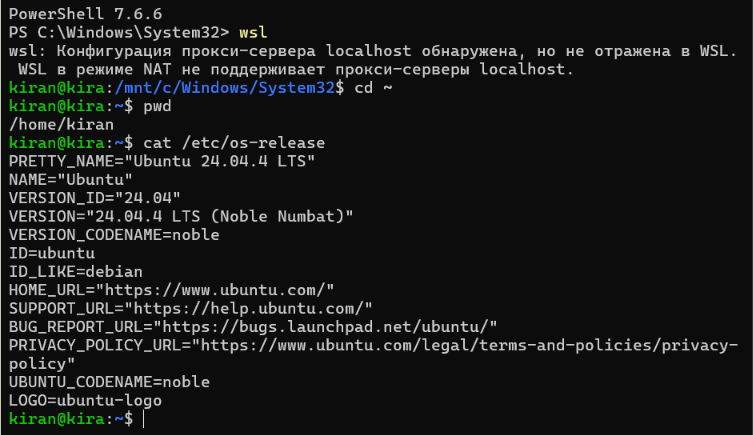
\includegraphics[width=0.7\linewidth,height=\textheight,keepaspectratio]{image/1.png}

}

\caption{Работа в Ubuntu через WSL}

\end{figure}%

\section{Настройка
Git}\label{ux43dux430ux441ux442ux440ux43eux439ux43aux430-git}

Для работы с репозиториями я настроила Git. В качестве имени
пользователя было указано \texttt{Kira\ Nechaeva}, а для GitHub и
GitVerse использовался общий адрес \texttt{knechaeva.git@gmail.com}.

Также были настроены SSH- и GPG-ключи и выполнена авторизация GitHub
CLI.

\begin{figure}[H]

{\centering 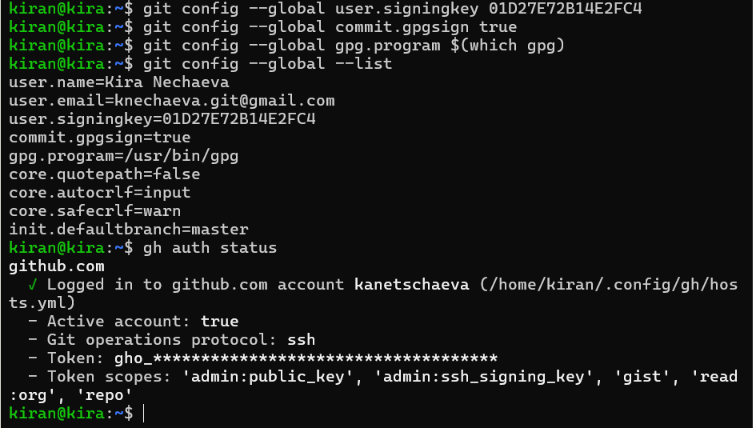
\includegraphics[width=0.7\linewidth,height=\textheight,keepaspectratio]{image/2.png}

}

\caption{Настройка Git и авторизация}

\end{figure}%

\section{Создание репозитория
GitVerse}\label{ux441ux43eux437ux434ux430ux43dux438ux435-ux440ux435ux43fux43eux437ux438ux442ux43eux440ux438ux44f-gitverse}

На основе шаблона курса в GitVerse был создан публичный репозиторий
\texttt{2026-1-\/-study-\/-mathmod}.

\begin{figure}[H]

{\centering 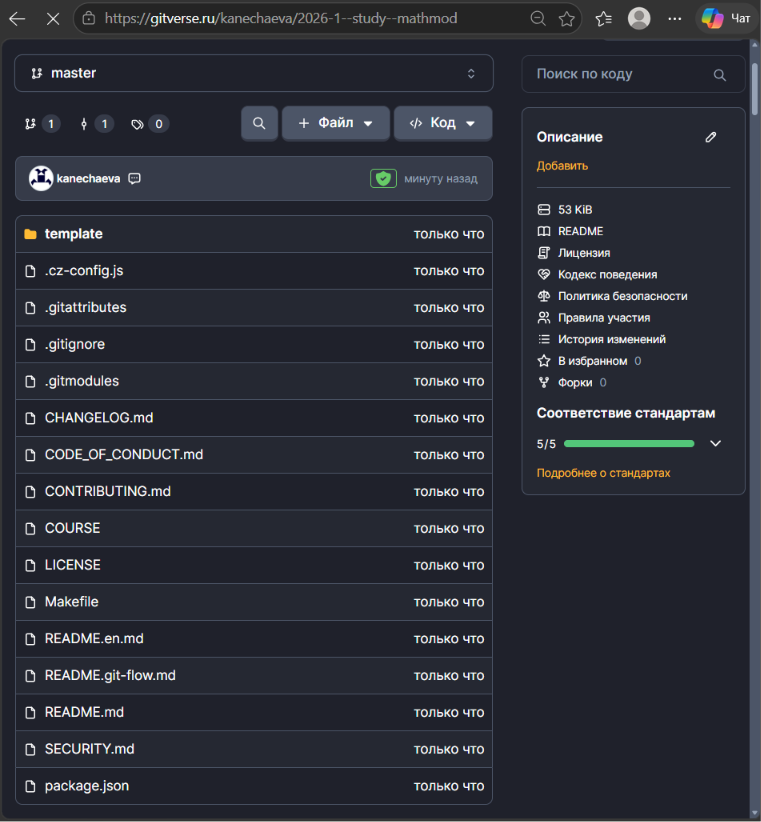
\includegraphics[width=0.7\linewidth,height=\textheight,keepaspectratio]{image/3.png}

}

\caption{Репозиторий курса в GitVerse}

\end{figure}%

После этого был создан рабочий каталог курса и репозиторий был
клонирован по SSH.

\begin{figure}[H]

{\centering 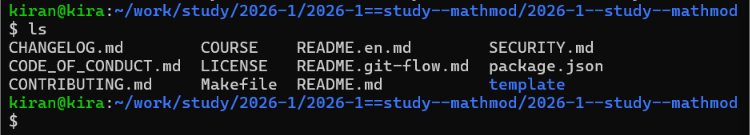
\includegraphics[width=0.7\linewidth,height=\textheight,keepaspectratio]{image/4.png}

}

\caption{Клонирование репозитория}

\end{figure}%

\section{Подготовка структуры
курса}\label{ux43fux43eux434ux433ux43eux442ux43eux432ux43aux430-ux441ux442ux440ux443ux43aux442ux443ux440ux44b-ux43aux443ux440ux441ux430}

Для настройки курса был создан файл \texttt{COURSE}, содержащий значение
\texttt{mathmod}, после чего была выполнена команда:

make prepare

Полученные изменения были добавлены в Git и отправлены в GitVerse.

\begin{figure}[H]

{\centering 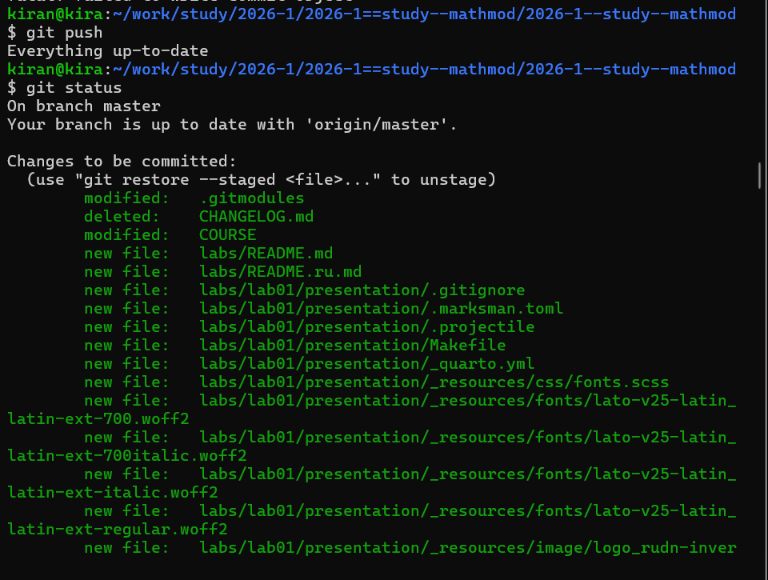
\includegraphics[width=0.7\linewidth,height=\textheight,keepaspectratio]{image/5.png}

}

\caption{make prepare + commit/push}

\end{figure}%

\section{Создание копии репозитория в
GitHub}\label{ux441ux43eux437ux434ux430ux43dux438ux435-ux43aux43eux43fux438ux438-ux440ux435ux43fux43eux437ux438ux442ux43eux440ux438ux44f-ux432-github}

Дополнительно был создан публичный репозиторий
\texttt{2026-1-\/-study-\/-mathmod} в GitHub.

\begin{figure}[H]

{\centering 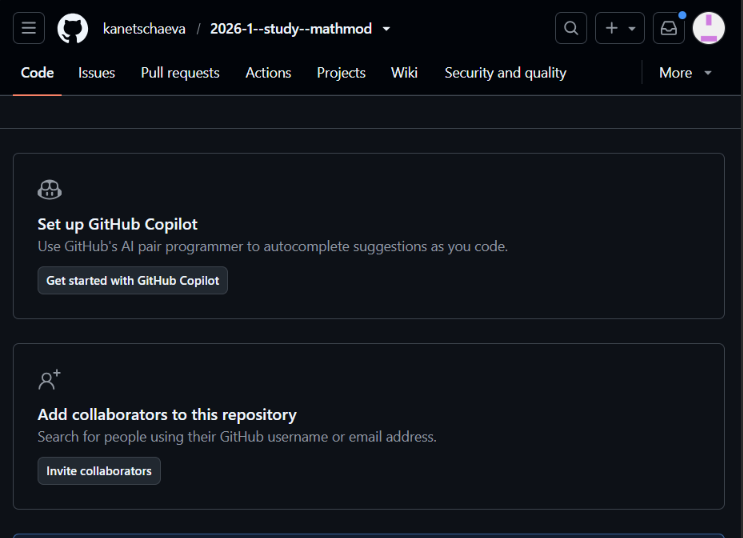
\includegraphics[width=0.7\linewidth,height=\textheight,keepaspectratio]{image/6.png}

}

\caption{Репозиторий в GitHub}

\end{figure}%

GitHub был добавлен как второй удалённый репозиторий с именем
\texttt{github}, после чего ветка \texttt{master} была отправлена в
него.

\begin{figure}[H]

{\centering 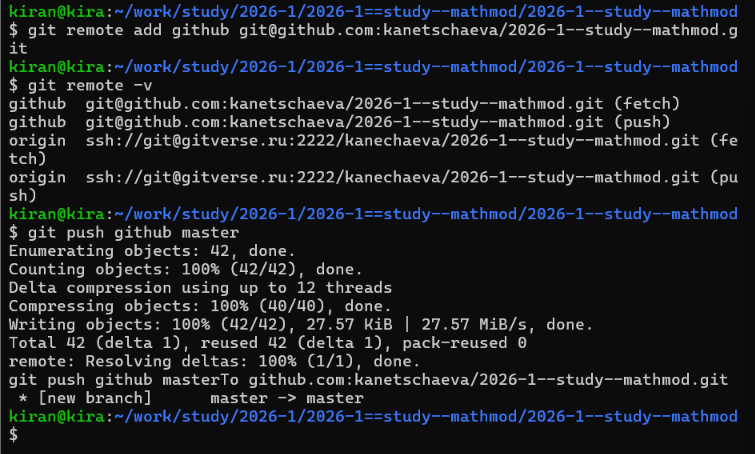
\includegraphics[width=0.7\linewidth,height=\textheight,keepaspectratio]{image/7.png}

}

\caption{Удалённые репозитории Git}

\end{figure}%

\section{Настройка Git
Flow}\label{ux43dux430ux441ux442ux440ux43eux439ux43aux430-git-flow}

Для организации разработки был инициализирован Git Flow. Основной веткой
является \texttt{master}, веткой разработки - \texttt{develop}, а
префиксом тегов выбран \texttt{v}.

После этого был создан первый релиз \texttt{1.0.0} и тег
\texttt{v1.0.0}.

\begin{figure}[H]

{\centering 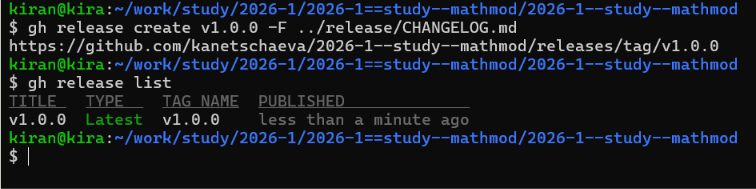
\includegraphics[width=0.7\linewidth,height=\textheight,keepaspectratio]{image/8.png}

}

\caption{Создание релиза с помощью Git Flow}

\end{figure}%

\section{Создание рабочего пространства лабораторной
работы}\label{ux441ux43eux437ux434ux430ux43dux438ux435-ux440ux430ux431ux43eux447ux435ux433ux43e-ux43fux440ux43eux441ux442ux440ux430ux43dux441ux442ux432ux430-ux43bux430ux431ux43eux440ux430ux442ux43eux440ux43dux43eux439-ux440ux430ux431ux43eux442ux44b}

В каталоге \texttt{labs} был создан каталог \texttt{lab01}. В нём
находятся каталоги проекта, отчёта и презентации.

\begin{figure}[H]

{\centering 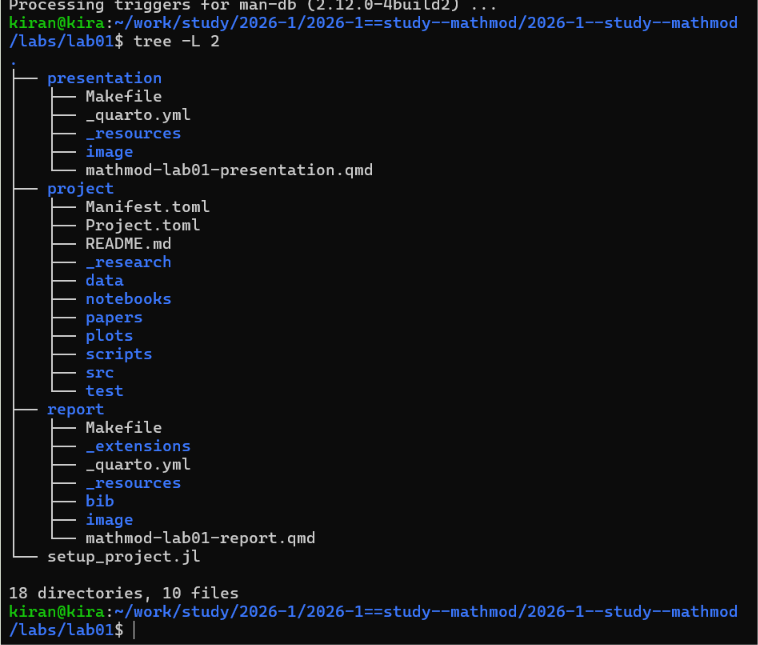
\includegraphics[width=0.7\linewidth,height=\textheight,keepaspectratio]{image/9.png}

}

\caption{Структура каталога lab01}

\end{figure}%

\section{Создание проекта
DrWatson}\label{ux441ux43eux437ux434ux430ux43dux438ux435-ux43fux440ux43eux435ux43aux442ux430-drwatson}

В каталоге первой лабораторной работы был создан проект DrWatson с
именем \texttt{project}.

\begin{figure}[H]

{\centering 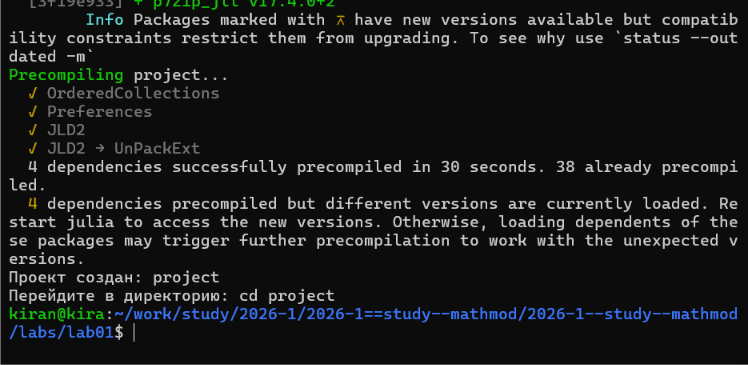
\includegraphics[width=0.7\linewidth,height=\textheight,keepaspectratio]{image/10.png}

}

\caption{Создание проекта DrWatson}

\end{figure}%

\section{Установка необходимых
пакетов}\label{ux443ux441ux442ux430ux43dux43eux432ux43aux430-ux43dux435ux43eux431ux445ux43eux434ux438ux43cux44bux445-ux43fux430ux43aux435ux442ux43eux432}

В окружение проекта были установлены пакеты DrWatson,
DifferentialEquations, Plots, DataFrames, CSV, JLD2, Literate, IJulia,
BenchmarkTools и Quarto.

\begin{figure}[H]

{\centering 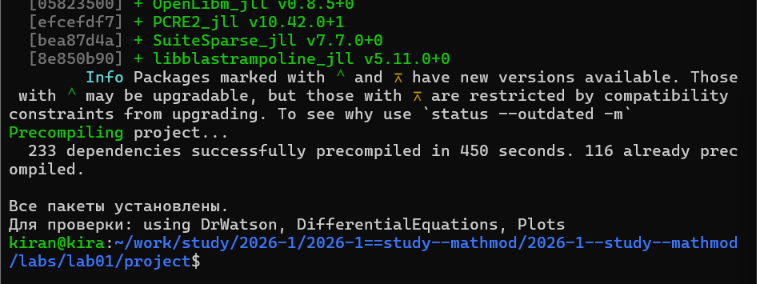
\includegraphics[width=0.7\linewidth,height=\textheight,keepaspectratio]{image/11.png}

}

\caption{Установка пакетов Julia}

\end{figure}%

После установки была выполнена проверка загрузки основных пакетов.

\begin{figure}[H]

{\centering 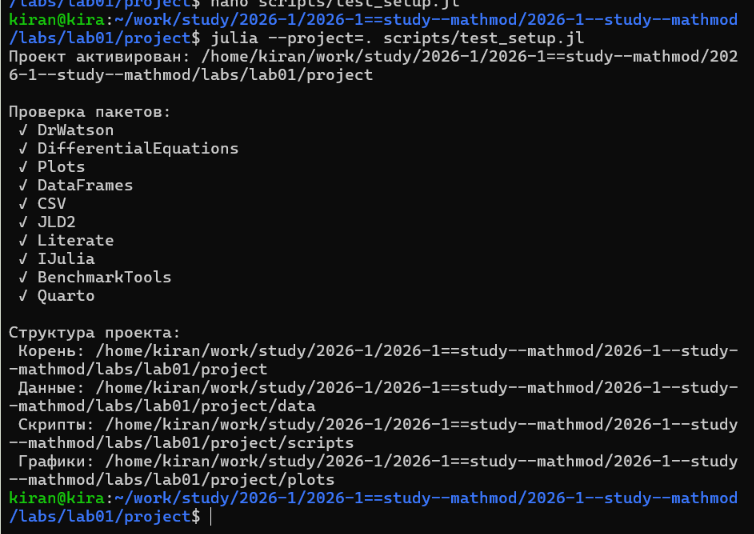
\includegraphics[width=0.7\linewidth,height=\textheight,keepaspectratio]{image/12.png}

}

\caption{Проверка пакетов}

\end{figure}%

\chapter{Модель экспоненциального
роста}\label{ux43cux43eux434ux435ux43bux44c-ux44dux43aux441ux43fux43eux43dux435ux43dux446ux438ux430ux43bux44cux43dux43eux433ux43e-ux440ux43eux441ux442ux430}

Экспоненциальный рост описывается дифференциальным уравнением

\[
\frac{du}{dt} = \alpha u.
\]

Для первого эксперимента использовались начальное значение
\texttt{u(0)=1}, коэффициент роста \texttt{α=0.3} и временной интервал
от 0 до 10.

Для решения задачи использовался пакет DifferentialEquations и метод
Tsit5.

\begin{figure}[H]

{\centering 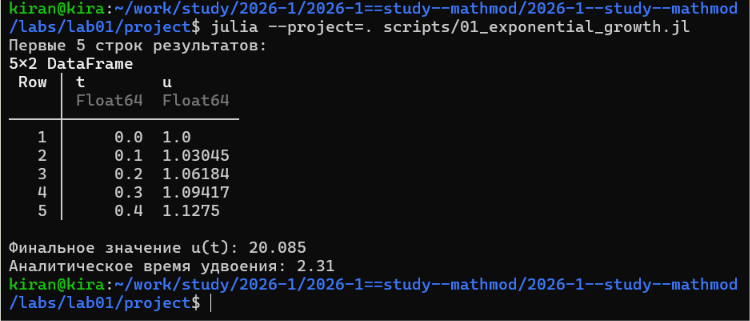
\includegraphics[width=0.7\linewidth,height=\textheight,keepaspectratio]{image/13.png}

}

\caption{Запуск модели экспоненциального роста}

\end{figure}%

В результате был построен график изменения величины \texttt{u(t)}.

\begin{figure}[H]

{\centering 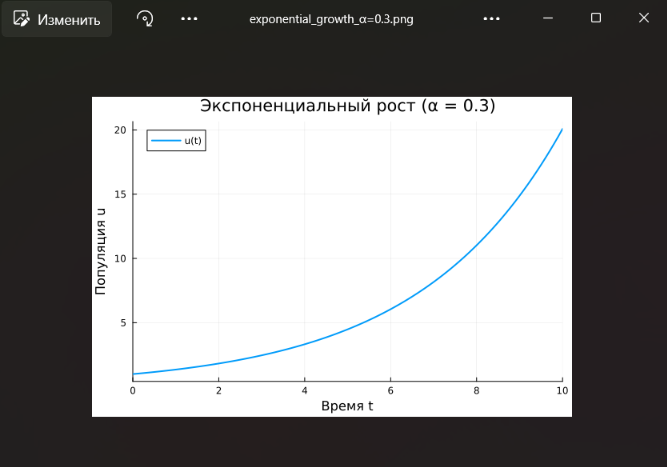
\includegraphics[width=0.7\linewidth,height=\textheight,keepaspectratio]{image/14.png}

}

\caption{График экспоненциального роста}

\end{figure}%

Время удвоения определяется по формуле

\[
t_2=\frac{\ln 2}{\alpha}.
\]

При \texttt{α=0.3} оно составляет примерно \texttt{2.31}.

\section{Преобразование программы в литературный
стиль}\label{ux43fux440ux435ux43eux431ux440ux430ux437ux43eux432ux430ux43dux438ux435-ux43fux440ux43eux433ux440ux430ux43cux43cux44b-ux432-ux43bux438ux442ux435ux440ux430ux442ux443ux440ux43dux44bux439-ux441ux442ux438ux43bux44c}

После первого запуска программа была преобразована в литературный стиль.
В код были добавлены поясняющие разделы, а результаты стали сохраняться
в стандартные каталоги проекта DrWatson.

\begin{figure}[H]

{\centering 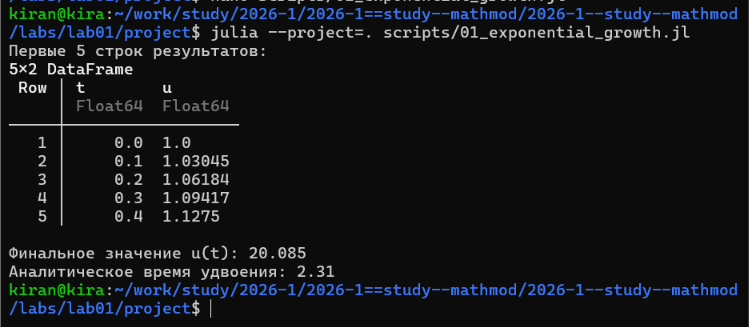
\includegraphics[width=0.7\linewidth,height=\textheight,keepaspectratio]{image/15.png}

}

\caption{Выполнение литературного кода}

\end{figure}%

\section{Генерация производных
форматов}\label{ux433ux435ux43dux435ux440ux430ux446ux438ux44f-ux43fux440ux43eux438ux437ux432ux43eux434ux43dux44bux445-ux444ux43eux440ux43cux430ux442ux43eux432}

При помощи Literate.jl из литературного исходного кода были
сгенерированы:

\begin{itemize}
\tightlist
\item
  чистый Julia-код;
\item
  документ Quarto;
\item
  Jupyter notebook.
\end{itemize}

\begin{figure}[H]

{\centering 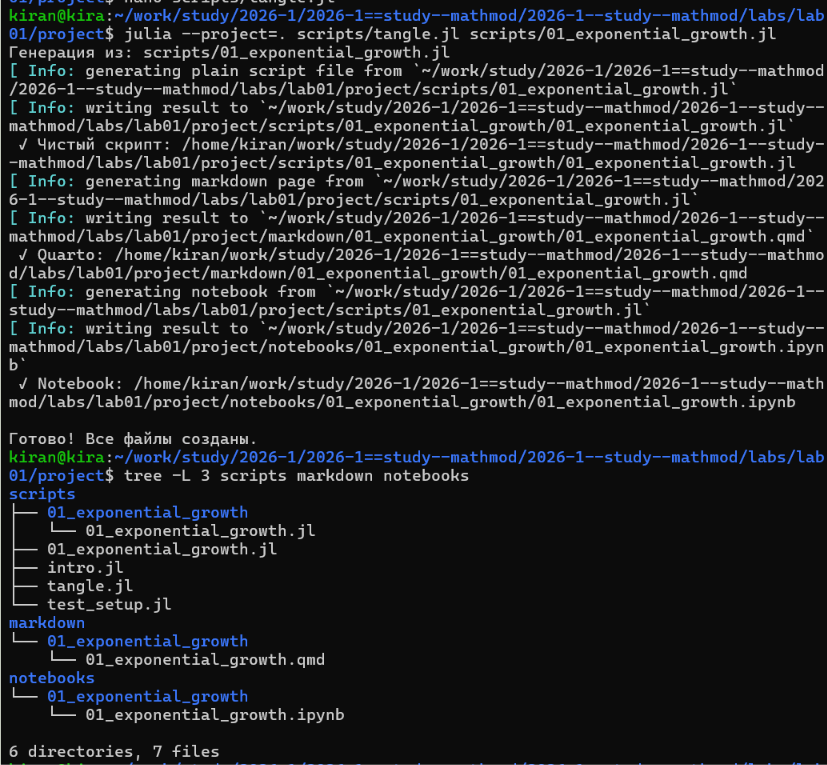
\includegraphics[width=0.7\linewidth,height=\textheight,keepaspectratio]{image/16.png}

}

\caption{Генерация производных форматов}

\end{figure}%

\section{Выполнение Jupyter
notebook}\label{ux432ux44bux43fux43eux43bux43dux435ux43dux438ux435-jupyter-notebook}

Сгенерированный notebook \texttt{01\_exponential\_growth.ipynb} был
открыт в Jupyter и выполнен.

\begin{figure}[H]

{\centering 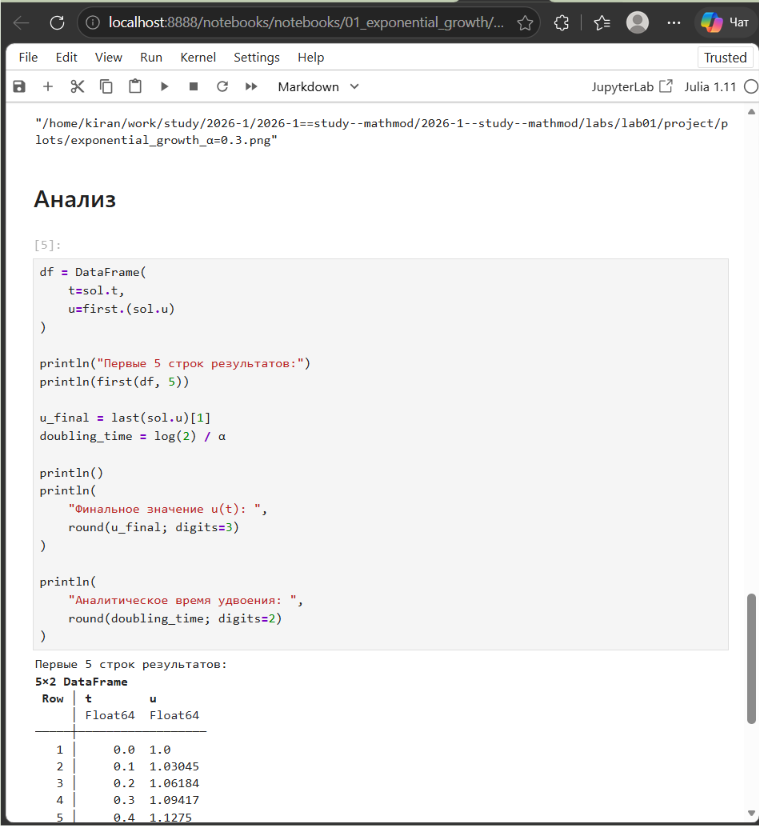
\includegraphics[width=0.7\linewidth,height=\textheight,keepaspectratio]{image/17.png}

}

\caption{Выполнение первого Jupyter notebook}

\end{figure}%

\section{Интеграция документации модели в
отчёт}\label{ux438ux43dux442ux435ux433ux440ux430ux446ux438ux44f-ux434ux43eux43aux443ux43cux435ux43dux442ux430ux446ux438ux438-ux43cux43eux434ux435ux43bux438-ux432-ux43eux442ux447ux451ux442}

В отчёт была подключена документация, автоматически сгенерированная из
литературного Julia-кода.

\chapter{Экспоненциальный
рост}\label{ux44dux43aux441ux43fux43eux43dux435ux43dux446ux438ux430ux43bux44cux43dux44bux439-ux440ux43eux441ux442}

\textbf{Цель:} исследовать решение уравнения du/dt = αu.

Экспоненциальный рост - это процесс увеличения величины, при котором
скорость роста в каждый момент времени пропорциональна текущему значению
этой величины.

\begin{Shaded}
\begin{Highlighting}[]
\ImportTok{using} \BuiltInTok{DrWatson}
\PreprocessorTok{@quickactivate} \StringTok{"project"}

\ImportTok{using} \BuiltInTok{DifferentialEquations}
\ImportTok{using} \BuiltInTok{Plots}
\ImportTok{using} \BuiltInTok{DataFrames}
\ImportTok{using} \BuiltInTok{JLD2}

\NormalTok{script\_name }\OperatorTok{=} \FunctionTok{splitext}\NormalTok{(}\FunctionTok{basename}\NormalTok{(}\ConstantTok{PROGRAM\_FILE}\NormalTok{))[}\FloatTok{1}\NormalTok{]}

\FunctionTok{mkpath}\NormalTok{(}\FunctionTok{plotsdir}\NormalTok{(script\_name))}
\FunctionTok{mkpath}\NormalTok{(}\FunctionTok{datadir}\NormalTok{(script\_name))}
\end{Highlighting}
\end{Shaded}

\begin{verbatim}
"/home/kiran/work/study/2026-1/2026-1==study--mathmod/2026-1--study--mathmod/labs/lab01/project/data/startup"
\end{verbatim}

\section{Определение
модели}\label{ux43eux43fux440ux435ux434ux435ux43bux435ux43dux438ux435-ux43cux43eux434ux435ux43bux438}

\begin{Shaded}
\begin{Highlighting}[]
\KeywordTok{function} \FunctionTok{exponential\_growth!}\NormalTok{(du, u, p, t)}
\NormalTok{    α }\OperatorTok{=}\NormalTok{ p}
\NormalTok{    du[}\FloatTok{1}\NormalTok{] }\OperatorTok{=}\NormalTok{ α }\OperatorTok{*}\NormalTok{ u[}\FloatTok{1}\NormalTok{]}
\KeywordTok{end}
\end{Highlighting}
\end{Shaded}

\begin{verbatim}
exponential_growth! (generic function with 1 method)
\end{verbatim}

\section{Первый
запуск}\label{ux43fux435ux440ux432ux44bux439-ux437ux430ux43fux443ux441ux43a}

\begin{Shaded}
\begin{Highlighting}[]
\NormalTok{u0 }\OperatorTok{=}\NormalTok{ [}\FloatTok{1.0}\NormalTok{]}
\NormalTok{α }\OperatorTok{=} \FloatTok{0.3}
\NormalTok{tspan }\OperatorTok{=}\NormalTok{ (}\FloatTok{0.0}\NormalTok{, }\FloatTok{10.0}\NormalTok{)}

\NormalTok{prob }\OperatorTok{=} \FunctionTok{ODEProblem}\NormalTok{(}
\NormalTok{    exponential\_growth!,}
\NormalTok{    u0,}
\NormalTok{    tspan,}
\NormalTok{    α}
\NormalTok{)}

\NormalTok{sol }\OperatorTok{=} \FunctionTok{solve}\NormalTok{(}
\NormalTok{    prob,}
    \FunctionTok{Tsit5}\NormalTok{(),}
\NormalTok{    saveat}\OperatorTok{=}\FloatTok{0.1}
\NormalTok{)}
\end{Highlighting}
\end{Shaded}

\begin{verbatim}
retcode: Success
Interpolation: 1st order linear
t: 101-element Vector{Float64}:
  0.0
  0.1
  0.2
  0.3
  0.4
  0.5
  0.6
  0.7
  0.8
  0.9
  ⋮
  9.2
  9.3
  9.4
  9.5
  9.6
  9.7
  9.8
  9.9
 10.0
u: 101-element Vector{Vector{Float64}}:
 [1.0]
 [1.030454533950446]
 [1.0618365551529674]
 [1.09417430287941]
 [1.1274968605386673]
 [1.1618342327450653]
 [1.1972173476990624]
 [1.233678057187257]
 [1.2712491879500347]
 [1.3099646073864082]
 ⋮
 [15.799688704153066]
 [16.280848966976624]
 [16.776672166300507]
 [17.287605875776954]
 [17.814109831385316]
 [18.35665593143256]
 [18.915728236552802]
 [19.491822969707872]
 [20.085448516186737]
\end{verbatim}

\section{Визуализация}\label{ux432ux438ux437ux443ux430ux43bux438ux437ux430ux446ux438ux44f}

\begin{Shaded}
\begin{Highlighting}[]
\FunctionTok{plot}\NormalTok{(}
\NormalTok{    sol,}
\NormalTok{    label}\OperatorTok{=}\StringTok{"u(t)"}\NormalTok{,}
\NormalTok{    xlabel}\OperatorTok{=}\StringTok{"Время t"}\NormalTok{,}
\NormalTok{    ylabel}\OperatorTok{=}\StringTok{"Популяция u"}\NormalTok{,}
\NormalTok{    title}\OperatorTok{=}\StringTok{"Экспоненциальный рост (α = }\SpecialCharTok{$}\StringTok{α)",}
\StringTok{    }\NormalTok{lw}\StringTok{=2,}
\NormalTok{    legend}\OperatorTok{=:}\NormalTok{topleft}
\NormalTok{)}

\FunctionTok{savefig}\NormalTok{(}
    \FunctionTok{plotsdir}\NormalTok{(}
\NormalTok{        script\_name,}
        \StringTok{"exponential\_growth\_α=}\SpecialCharTok{$}\StringTok{α.}\NormalTok{png}\StringTok{"}
\NormalTok{    )}
\NormalTok{)}
\end{Highlighting}
\end{Shaded}

\begin{verbatim}
"/home/kiran/work/study/2026-1/2026-1==study--mathmod/2026-1--study--mathmod/labs/lab01/project/plots/startup/exponential_growth_α=0.3.png"
\end{verbatim}

\section{Анализ}\label{ux430ux43dux430ux43bux438ux437}

\begin{Shaded}
\begin{Highlighting}[]
\NormalTok{df }\OperatorTok{=} \FunctionTok{DataFrame}\NormalTok{(}
\NormalTok{    t}\OperatorTok{=}\NormalTok{sol.t,}
\NormalTok{    u}\OperatorTok{=}\FunctionTok{first}\NormalTok{.(sol.u)}
\NormalTok{)}

\FunctionTok{println}\NormalTok{(}\StringTok{"Первые 5 строк результатов:"}\NormalTok{)}
\FunctionTok{println}\NormalTok{(}\FunctionTok{first}\NormalTok{(df, }\FloatTok{5}\NormalTok{))}

\NormalTok{u\_final }\OperatorTok{=} \FunctionTok{last}\NormalTok{(sol.u)[}\FloatTok{1}\NormalTok{]}
\NormalTok{doubling\_time }\OperatorTok{=} \FunctionTok{log}\NormalTok{(}\FloatTok{2}\NormalTok{) }\OperatorTok{/}\NormalTok{ α}

\FunctionTok{println}\NormalTok{()}
\FunctionTok{println}\NormalTok{(}
    \StringTok{"Финальное значение u(t): "}\NormalTok{,}
    \FunctionTok{round}\NormalTok{(u\_final; digits}\OperatorTok{=}\FloatTok{3}\NormalTok{)}
\NormalTok{)}

\FunctionTok{println}\NormalTok{(}
    \StringTok{"Аналитическое время удвоения: "}\NormalTok{,}
    \FunctionTok{round}\NormalTok{(doubling\_time; digits}\OperatorTok{=}\FloatTok{2}\NormalTok{)}
\NormalTok{)}
\end{Highlighting}
\end{Shaded}

\begin{verbatim}
Первые 5 строк результатов:
5×2 DataFrame
 Row │ t        u       
     │ Float64  Float64 
─────┼──────────────────
   1 │     0.0  1.0
   2 │     0.1  1.03045
   3 │     0.2  1.06184
   4 │     0.3  1.09417
   5 │     0.4  1.1275

Финальное значение u(t): 20.085
Аналитическое время удвоения: 2.31
\end{verbatim}

\section{Сохранение
результатов}\label{ux441ux43eux445ux440ux430ux43dux435ux43dux438ux435-ux440ux435ux437ux443ux43bux44cux442ux430ux442ux43eux432}

\begin{Shaded}
\begin{Highlighting}[]
\PreprocessorTok{@save} \FunctionTok{datadir}\NormalTok{(}
\NormalTok{    script\_name,}
    \StringTok{"all\_results.jld2"}
\NormalTok{) df}
\end{Highlighting}
\end{Shaded}

\begin{figure}[H]

{\centering 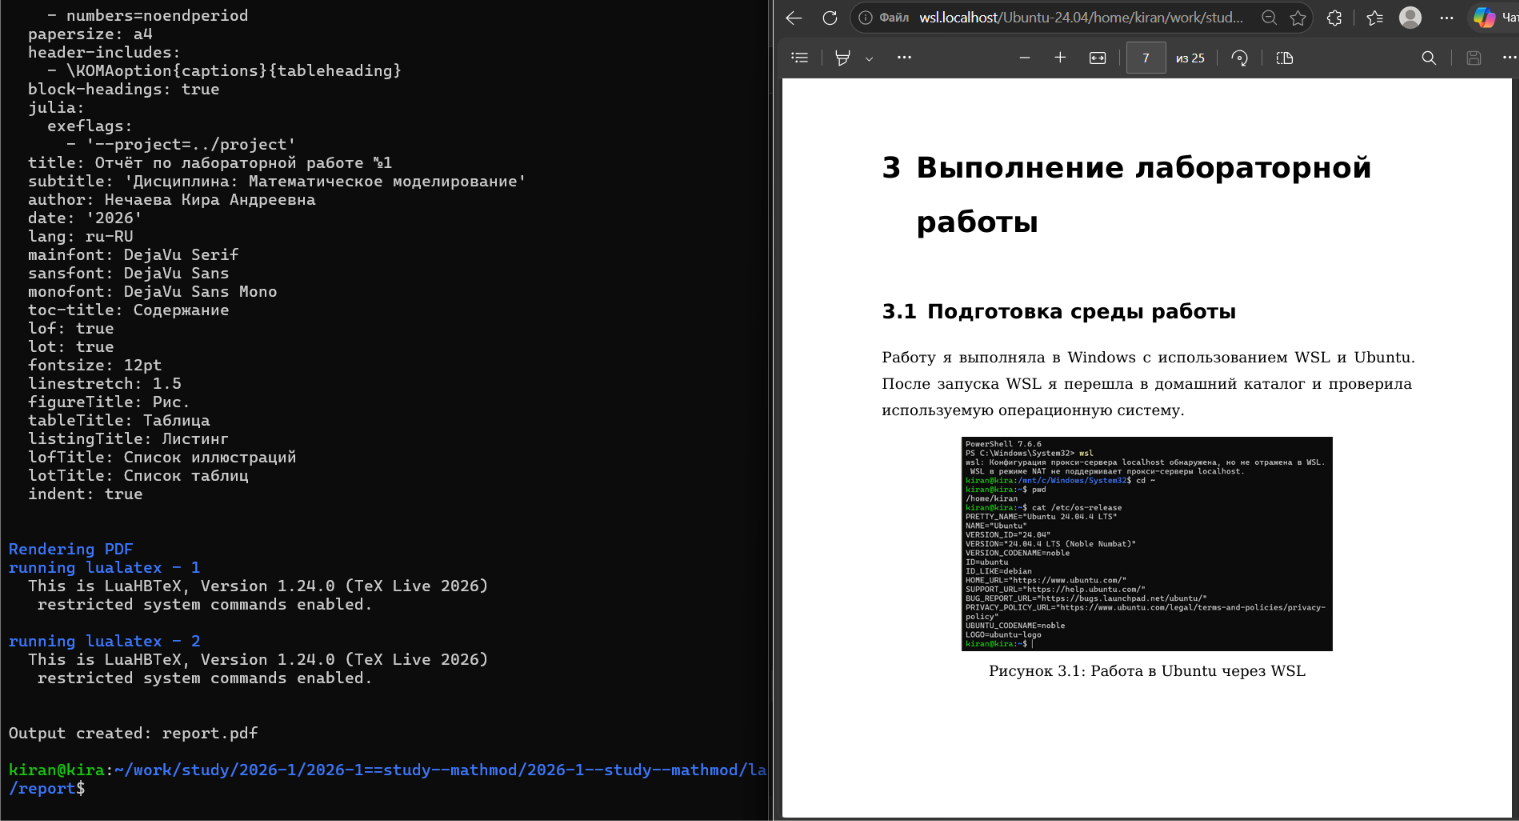
\includegraphics[width=0.7\linewidth,height=\textheight,keepaspectratio]{image/18.png}

}

\caption{Сборка отчёта после подключения первой документации}

\end{figure}%

\chapter{Параметрическое
исследование}\label{ux43fux430ux440ux430ux43cux435ux442ux440ux438ux447ux435ux441ux43aux43eux435-ux438ux441ux441ux43bux435ux434ux43eux432ux430ux43dux438ux435}

После исследования базового случая модель была дополнена возможностью
автоматического запуска для нескольких значений коэффициента роста.

Исследовались значения

α = 0.1, 0.3, 0.5, 0.8, 1.0.

Для каждого набора параметров программа решала задачу и сохраняла
полученные результаты.

\begin{figure}[H]

{\centering 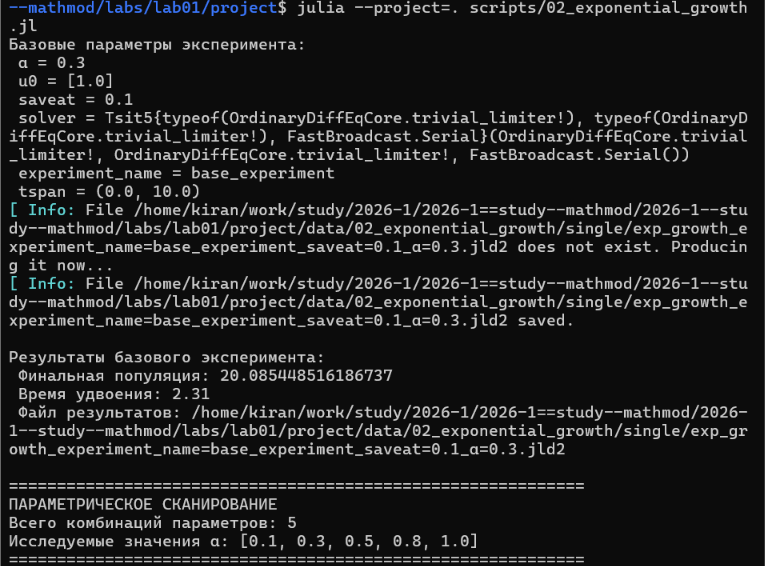
\includegraphics[width=0.7\linewidth,height=\textheight,keepaspectratio]{image/19.png}

}

\caption{Запуск параметрического исследования}

\end{figure}%

\section{Результаты параметрического
исследования}\label{ux440ux435ux437ux443ux43bux44cux442ux430ux442ux44b-ux43fux430ux440ux430ux43cux435ux442ux440ux438ux447ux435ux441ux43aux43eux433ux43e-ux438ux441ux441ux43bux435ux434ux43eux432ux430ux43dux438ux44f}

Полученные результаты были собраны в общую таблицу.

\begin{figure}[H]

{\centering 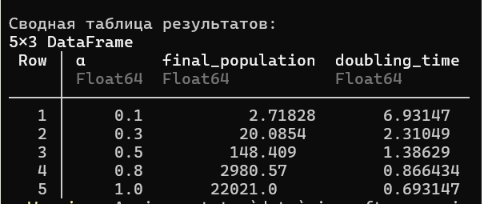
\includegraphics[width=0.7\linewidth,height=\textheight,keepaspectratio]{image/20.png}

}

\caption{Сводная таблица результатов}

\end{figure}%

При увеличении коэффициента \texttt{α} значение функции в конце
рассматриваемого интервала быстро увеличивается. Одновременно
уменьшается время удвоения.

\section{Сравнение
результатов}\label{ux441ux440ux430ux432ux43dux435ux43dux438ux435-ux440ux435ux437ux443ux43bux44cux442ux430ux442ux43eux432}

Для сравнения были построены траектории решения при всех исследованных
значениях коэффициента роста.

\begin{figure}[H]

{\centering 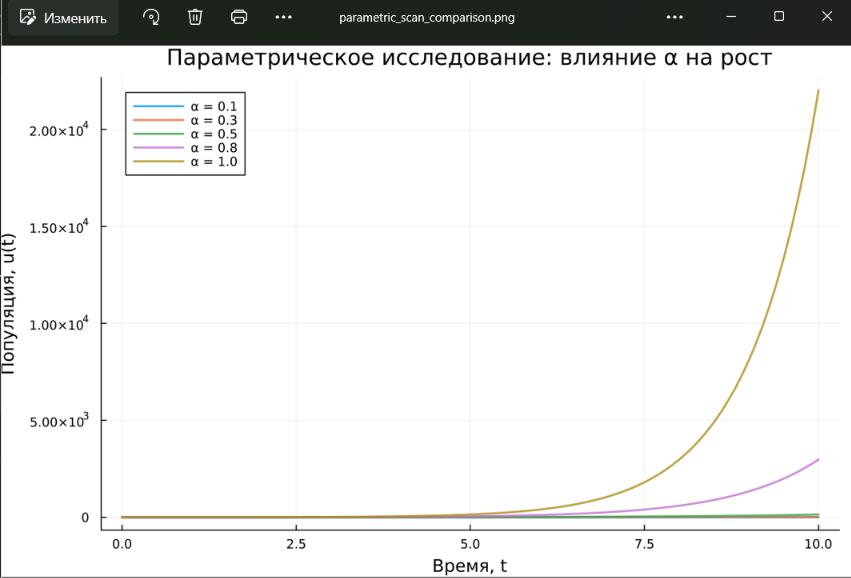
\includegraphics[width=0.7\linewidth,height=\textheight,keepaspectratio]{image/21.png}

}

\caption{Сравнение траекторий}

\end{figure}%

Также была построена зависимость времени удвоения от коэффициента роста.

\begin{figure}[H]

{\centering 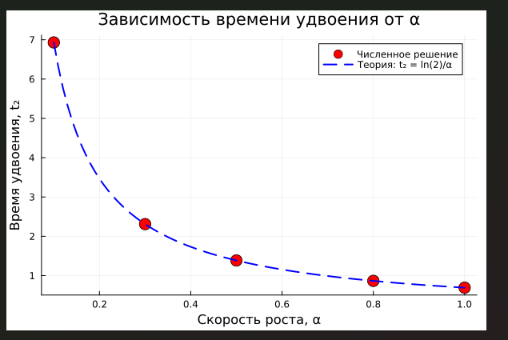
\includegraphics[width=0.7\linewidth,height=\textheight,keepaspectratio]{image/22.png}

}

\caption{Зависимость времени удвоения от alpha}

\end{figure}%

\section{Бенчмаркинг}\label{ux431ux435ux43dux447ux43cux430ux440ux43aux438ux43dux433}

Для оценки времени решения модели был выполнен бенчмаркинг для каждого
исследуемого значения \texttt{α}.

\begin{figure}[H]

{\centering 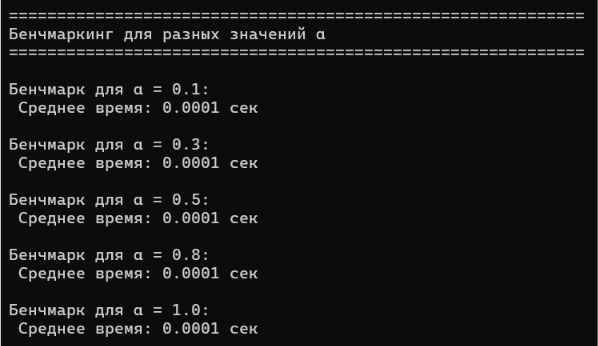
\includegraphics[width=0.7\linewidth,height=\textheight,keepaspectratio]{image/23.png}

}

\caption{Результаты бенчмаркинга}

\end{figure}%

По полученным данным был построен график зависимости времени вычисления
от значения параметра.

\begin{figure}[H]

{\centering 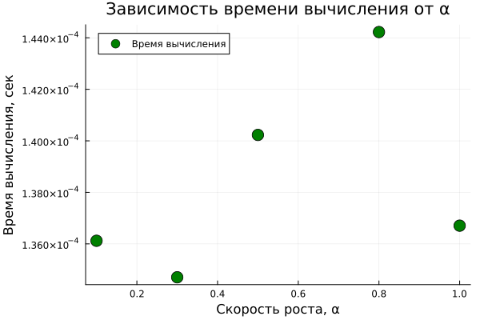
\includegraphics[width=0.7\linewidth,height=\textheight,keepaspectratio]{image/24.png}

}

\caption{Время вычисления модели}

\end{figure}%

\section{Генерация форматов параметрического
кода}\label{ux433ux435ux43dux435ux440ux430ux446ux438ux44f-ux444ux43eux440ux43cux430ux442ux43eux432-ux43fux430ux440ux430ux43cux435ux442ux440ux438ux447ux435ux441ux43aux43eux433ux43e-ux43aux43eux434ux430}

Для параметрической версии программы также были сгенерированы чистый
Julia-код, Quarto-документ и Jupyter notebook.

\begin{figure}[H]

{\centering 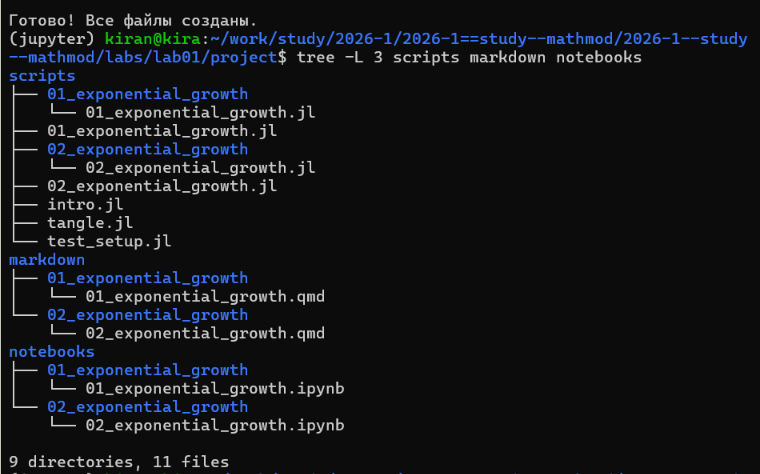
\includegraphics[width=0.7\linewidth,height=\textheight,keepaspectratio]{image/25.png}

}

\caption{Производные форматы параметрической модели}

\end{figure}%

\section{Выполнение параметрического
notebook}\label{ux432ux44bux43fux43eux43bux43dux435ux43dux438ux435-ux43fux430ux440ux430ux43cux435ux442ux440ux438ux447ux435ux441ux43aux43eux433ux43e-notebook}

Сгенерированный notebook \texttt{02\_exponential\_growth.ipynb} был
выполнен в Jupyter.

\begin{figure}[H]

{\centering 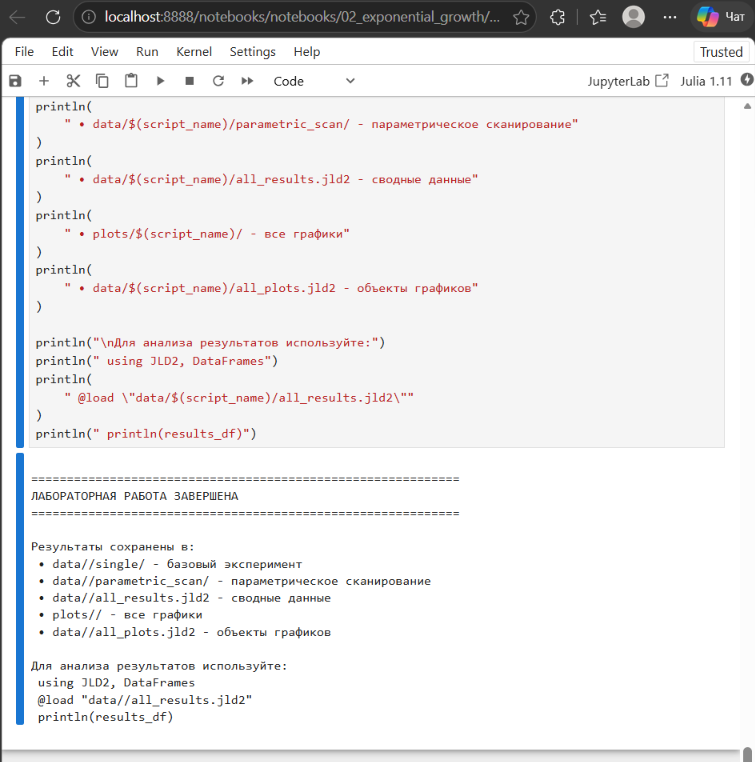
\includegraphics[width=0.7\linewidth,height=\textheight,keepaspectratio]{image/26.png}

}

\caption{Выполнение второго Jupyter notebook}

\end{figure}%

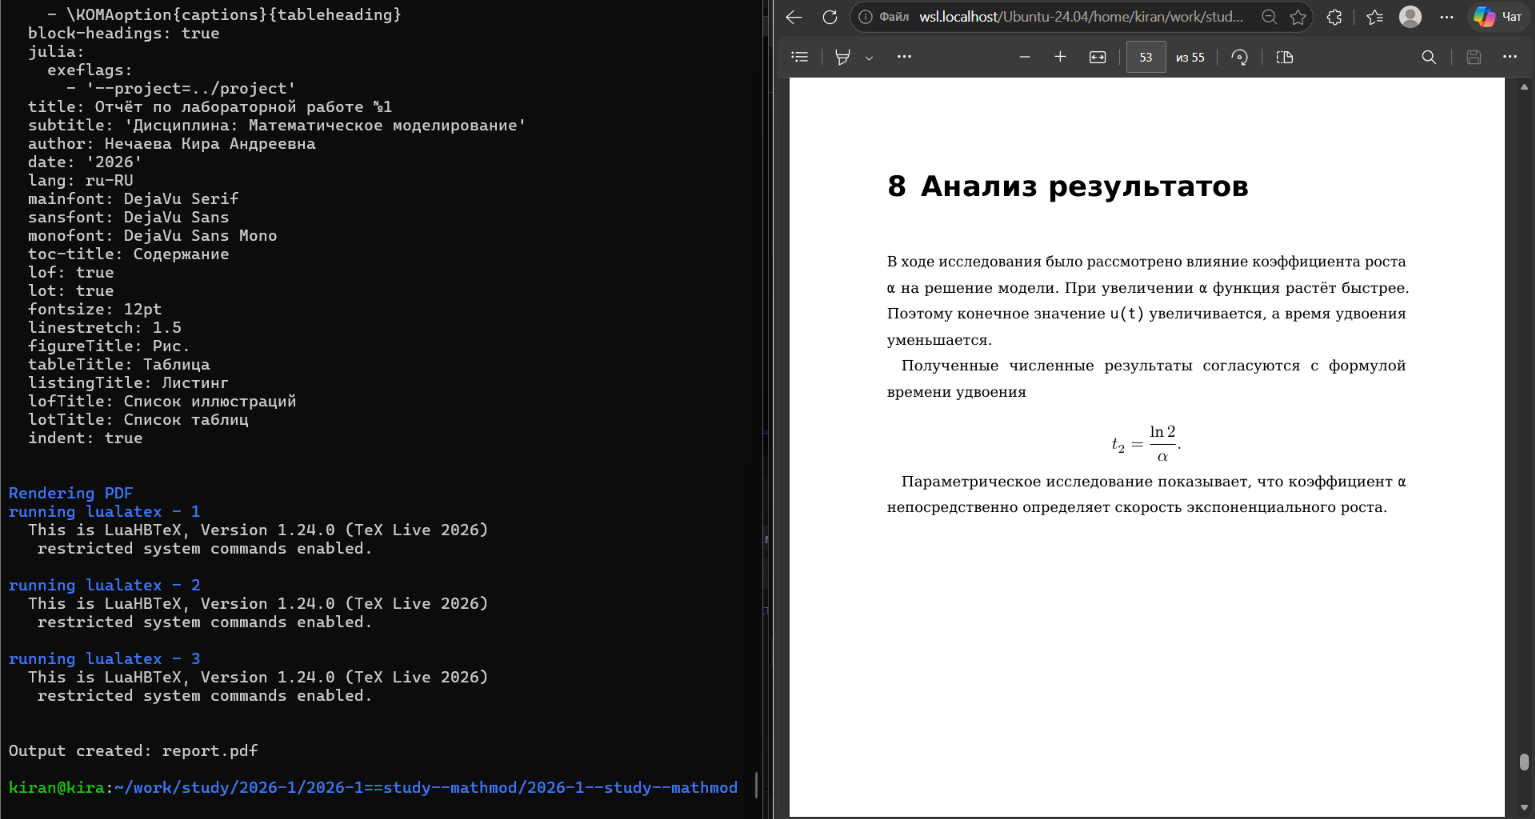
\includegraphics[width=0.7\linewidth,height=\textheight,keepaspectratio,alt={Итоговая сборка отчёта}]{image/27.png}\#\#
Интеграция документации параметрической модели

Документация параметрической версии модели также была автоматически
сгенерирована из литературного кода и подключена к отчёту.

\chapter{Параметрическое исследование экспоненциального
роста}\label{ux43fux430ux440ux430ux43cux435ux442ux440ux438ux447ux435ux441ux43aux43eux435-ux438ux441ux441ux43bux435ux434ux43eux432ux430ux43dux438ux435-ux44dux43aux441ux43fux43eux43dux435ux43dux446ux438ux430ux43bux44cux43dux43eux433ux43e-ux440ux43eux441ux442ux430}

\section{Активация проекта и загрузка
пакетов}\label{ux430ux43aux442ux438ux432ux430ux446ux438ux44f-ux43fux440ux43eux435ux43aux442ux430-ux438-ux437ux430ux433ux440ux443ux437ux43aux430-ux43fux430ux43aux435ux442ux43eux432}

\begin{Shaded}
\begin{Highlighting}[]
\ImportTok{using} \BuiltInTok{DrWatson}
\PreprocessorTok{@quickactivate} \StringTok{"project"}

\ImportTok{using} \BuiltInTok{DifferentialEquations}
\ImportTok{using} \BuiltInTok{DataFrames}
\ImportTok{using} \BuiltInTok{Plots}
\ImportTok{using} \BuiltInTok{JLD2}
\ImportTok{using} \BuiltInTok{BenchmarkTools}
\end{Highlighting}
\end{Shaded}

Установка каталогов

\begin{Shaded}
\begin{Highlighting}[]
\NormalTok{script\_name }\OperatorTok{=} \FunctionTok{splitext}\NormalTok{(}\FunctionTok{basename}\NormalTok{(}\ConstantTok{PROGRAM\_FILE}\NormalTok{))[}\FloatTok{1}\NormalTok{]}

\FunctionTok{mkpath}\NormalTok{(}\FunctionTok{plotsdir}\NormalTok{(script\_name))}
\FunctionTok{mkpath}\NormalTok{(}\FunctionTok{datadir}\NormalTok{(script\_name))}
\end{Highlighting}
\end{Shaded}

\begin{verbatim}
"/home/kiran/work/study/2026-1/2026-1==study--mathmod/2026-1--study--mathmod/labs/lab01/project/data/startup"
\end{verbatim}

\section{Определение
модели}\label{ux43eux43fux440ux435ux434ux435ux43bux435ux43dux438ux435-ux43cux43eux434ux435ux43bux438-1}

Модель: du/dt = α * u

\begin{Shaded}
\begin{Highlighting}[]
\KeywordTok{function} \FunctionTok{exponential\_growth!}\NormalTok{(du, u, p, t)}
\NormalTok{    α }\OperatorTok{=}\NormalTok{ p.α}
\NormalTok{    du[}\FloatTok{1}\NormalTok{] }\OperatorTok{=}\NormalTok{ α }\OperatorTok{*}\NormalTok{ u[}\FloatTok{1}\NormalTok{]}
\KeywordTok{end}
\end{Highlighting}
\end{Shaded}

\begin{verbatim}
exponential_growth! (generic function with 1 method)
\end{verbatim}

\section{Определение параметров в
Dict}\label{ux43eux43fux440ux435ux434ux435ux43bux435ux43dux438ux435-ux43fux430ux440ux430ux43cux435ux442ux440ux43eux432-ux432-dict}

Базовый набор параметров

\begin{Shaded}
\begin{Highlighting}[]
\NormalTok{base\_params }\OperatorTok{=} \FunctionTok{Dict}\NormalTok{(}
    \OperatorTok{:}\NormalTok{u0 }\OperatorTok{=\textgreater{}}\NormalTok{ [}\FloatTok{1.0}\NormalTok{],}
    \OperatorTok{:}\NormalTok{α }\OperatorTok{=\textgreater{}} \FloatTok{0.3}\NormalTok{,}
    \OperatorTok{:}\NormalTok{tspan }\OperatorTok{=\textgreater{}}\NormalTok{ (}\FloatTok{0.0}\NormalTok{, }\FloatTok{10.0}\NormalTok{),}
    \OperatorTok{:}\NormalTok{solver }\OperatorTok{=\textgreater{}} \FunctionTok{Tsit5}\NormalTok{(),}
    \OperatorTok{:}\NormalTok{saveat }\OperatorTok{=\textgreater{}} \FloatTok{0.1}\NormalTok{,}
    \OperatorTok{:}\NormalTok{experiment\_name }\OperatorTok{=\textgreater{}} \StringTok{"base\_experiment"}
\NormalTok{)}

\FunctionTok{println}\NormalTok{(}\StringTok{"Базовые параметры эксперимента:"}\NormalTok{)}

\ControlFlowTok{for}\NormalTok{ (key, value) }\KeywordTok{in}\NormalTok{ base\_params}
    \FunctionTok{println}\NormalTok{(}\StringTok{" }\SpecialCharTok{$}\NormalTok{key}\StringTok{ = }\SpecialCharTok{$}\NormalTok{value}\StringTok{"}\NormalTok{)}
\ControlFlowTok{end}
\end{Highlighting}
\end{Shaded}

\begin{verbatim}
Базовые параметры эксперимента:
 α = 0.3
 u0 = [1.0]
 saveat = 0.1
 solver = OrdinaryDiffEqTsit5.Tsit5{typeof(OrdinaryDiffEqCore.trivial_limiter!), typeof(OrdinaryDiffEqCore.trivial_limiter!), FastBroadcast.Serial}(OrdinaryDiffEqCore.trivial_limiter!, OrdinaryDiffEqCore.trivial_limiter!, FastBroadcast.Serial())
 experiment_name = base_experiment
 tspan = (0.0, 10.0)
\end{verbatim}

\section{Функция для запуска одного
эксперимента}\label{ux444ux443ux43dux43aux446ux438ux44f-ux434ux43bux44f-ux437ux430ux43fux443ux441ux43aux430-ux43eux434ux43dux43eux433ux43e-ux44dux43aux441ux43fux435ux440ux438ux43cux435ux43dux442ux430}

\begin{Shaded}
\begin{Highlighting}[]
\KeywordTok{function} \FunctionTok{run\_single\_experiment}\NormalTok{(params}\OperatorTok{::}\DataTypeTok{Dict}\NormalTok{)}

    \PreprocessorTok{@unpack}\NormalTok{ u0, α, tspan, solver, saveat }\OperatorTok{=}\NormalTok{ params}

\NormalTok{    prob }\OperatorTok{=} \FunctionTok{ODEProblem}\NormalTok{(}
\NormalTok{        exponential\_growth!,}
\NormalTok{        u0,}
\NormalTok{        tspan,}
\NormalTok{        (α}\OperatorTok{=}\NormalTok{α,)}
\NormalTok{    )}

\NormalTok{    sol }\OperatorTok{=} \FunctionTok{solve}\NormalTok{(}
\NormalTok{        prob,}
\NormalTok{        solver;}
\NormalTok{        saveat}\OperatorTok{=}\NormalTok{saveat}
\NormalTok{    )}

\NormalTok{    final\_population }\OperatorTok{=} \FunctionTok{last}\NormalTok{(sol.u)[}\FloatTok{1}\NormalTok{]}
\NormalTok{    doubling\_time }\OperatorTok{=} \FunctionTok{log}\NormalTok{(}\FloatTok{2}\NormalTok{) }\OperatorTok{/}\NormalTok{ α}

    \ControlFlowTok{return} \FunctionTok{Dict}\NormalTok{(}
        \StringTok{"solution"} \OperatorTok{=\textgreater{}}\NormalTok{ sol,}
        \StringTok{"time\_points"} \OperatorTok{=\textgreater{}}\NormalTok{ sol.t,}
        \StringTok{"population\_values"} \OperatorTok{=\textgreater{}} \FunctionTok{first}\NormalTok{.(sol.u),}
        \StringTok{"final\_population"} \OperatorTok{=\textgreater{}}\NormalTok{ final\_population,}
        \StringTok{"doubling\_time"} \OperatorTok{=\textgreater{}}\NormalTok{ doubling\_time,}
        \StringTok{"parameters"} \OperatorTok{=\textgreater{}}\NormalTok{ params}
\NormalTok{    )}
\KeywordTok{end}
\end{Highlighting}
\end{Shaded}

\begin{verbatim}
run_single_experiment (generic function with 1 method)
\end{verbatim}

\section{Запуск базового
эксперимента}\label{ux437ux430ux43fux443ux441ux43a-ux431ux430ux437ux43eux432ux43eux433ux43e-ux44dux43aux441ux43fux435ux440ux438ux43cux435ux43dux442ux430}

\begin{Shaded}
\begin{Highlighting}[]
\NormalTok{data, path }\OperatorTok{=} \FunctionTok{produce\_or\_load}\NormalTok{(}
    \FunctionTok{datadir}\NormalTok{(script\_name, }\StringTok{"single"}\NormalTok{),}
\NormalTok{    base\_params,}
\NormalTok{    run\_single\_experiment,}
\NormalTok{    prefix}\OperatorTok{=}\StringTok{"exp\_growth"}\NormalTok{,}
\NormalTok{    tag}\OperatorTok{=}\ConstantTok{false}\NormalTok{,}
\NormalTok{    verbose}\OperatorTok{=}\ConstantTok{true}
\NormalTok{)}

\FunctionTok{println}\NormalTok{(}\StringTok{"}\SpecialCharTok{\textbackslash{}n}\StringTok{Результаты базового эксперимента:"}\NormalTok{)}
\FunctionTok{println}\NormalTok{(}\StringTok{" Финальная популяция: "}\NormalTok{, data[}\StringTok{"final\_population"}\NormalTok{])}
\FunctionTok{println}\NormalTok{(}
    \StringTok{" Время удвоения: "}\NormalTok{,}
    \FunctionTok{round}\NormalTok{(data[}\StringTok{"doubling\_time"}\NormalTok{]; digits}\OperatorTok{=}\FloatTok{2}\NormalTok{)}
\NormalTok{)}
\FunctionTok{println}\NormalTok{(}\StringTok{" Файл результатов: "}\NormalTok{, path)}
\end{Highlighting}
\end{Shaded}

\begin{verbatim}

Результаты базового эксперимента:
 Финальная популяция: 20.085448516186737
 Время удвоения: 2.31
 Файл результатов: /home/kiran/work/study/2026-1/2026-1==study--mathmod/2026-1--study--mathmod/labs/lab01/project/data/startup/single/exp_growth_experiment_name=base_experiment_saveat=0.1_α=0.3.jld2
\end{verbatim}

\section{Визуализация базового
эксперимента}\label{ux432ux438ux437ux443ux430ux43bux438ux437ux430ux446ux438ux44f-ux431ux430ux437ux43eux432ux43eux433ux43e-ux44dux43aux441ux43fux435ux440ux438ux43cux435ux43dux442ux430}

\begin{Shaded}
\begin{Highlighting}[]
\NormalTok{p1 }\OperatorTok{=} \FunctionTok{plot}\NormalTok{(}
\NormalTok{    data[}\StringTok{"time\_points"}\NormalTok{],}
\NormalTok{    data[}\StringTok{"population\_values"}\NormalTok{],}
\NormalTok{    label}\OperatorTok{=}\StringTok{"α = }\SpecialCharTok{$}\NormalTok{(base\_params[}\OperatorTok{:}\NormalTok{α])}\StringTok{"}\NormalTok{,}
\NormalTok{    xlabel}\OperatorTok{=}\StringTok{"Время, t"}\NormalTok{,}
\NormalTok{    ylabel}\OperatorTok{=}\StringTok{"Популяция, u(t)"}\NormalTok{,}
\NormalTok{    title}\OperatorTok{=}\StringTok{"Экспоненциальный рост (базовый эксперимент)"}\NormalTok{,}
\NormalTok{    lw}\OperatorTok{=}\FloatTok{2}\NormalTok{,}
\NormalTok{    legend}\OperatorTok{=:}\NormalTok{topleft,}
\NormalTok{    grid}\OperatorTok{=}\ConstantTok{true}
\NormalTok{)}

\FunctionTok{savefig}\NormalTok{(}
    \FunctionTok{plotsdir}\NormalTok{(}
\NormalTok{        script\_name,}
        \StringTok{"single\_experiment.png"}
\NormalTok{    )}
\NormalTok{)}
\end{Highlighting}
\end{Shaded}

\begin{verbatim}
"/home/kiran/work/study/2026-1/2026-1==study--mathmod/2026-1--study--mathmod/labs/lab01/project/plots/startup/single_experiment.png"
\end{verbatim}

\section{Параметрическое
сканирование}\label{ux43fux430ux440ux430ux43cux435ux442ux440ux438ux447ux435ux441ux43aux43eux435-ux441ux43aux430ux43dux438ux440ux43eux432ux430ux43dux438ux435}

\begin{Shaded}
\begin{Highlighting}[]
\NormalTok{param\_grid }\OperatorTok{=} \FunctionTok{Dict}\NormalTok{(}
    \OperatorTok{:}\NormalTok{u0 }\OperatorTok{=\textgreater{}}\NormalTok{ [[}\FloatTok{1.0}\NormalTok{]],}
    \OperatorTok{:}\NormalTok{α }\OperatorTok{=\textgreater{}}\NormalTok{ [}\FloatTok{0.1}\NormalTok{, }\FloatTok{0.3}\NormalTok{, }\FloatTok{0.5}\NormalTok{, }\FloatTok{0.8}\NormalTok{, }\FloatTok{1.0}\NormalTok{],}
    \OperatorTok{:}\NormalTok{tspan }\OperatorTok{=\textgreater{}}\NormalTok{ [(}\FloatTok{0.0}\NormalTok{, }\FloatTok{10.0}\NormalTok{)],}
    \OperatorTok{:}\NormalTok{solver }\OperatorTok{=\textgreater{}}\NormalTok{ [}\FunctionTok{Tsit5}\NormalTok{()],}
    \OperatorTok{:}\NormalTok{saveat }\OperatorTok{=\textgreater{}}\NormalTok{ [}\FloatTok{0.1}\NormalTok{],}
    \OperatorTok{:}\NormalTok{experiment\_name }\OperatorTok{=\textgreater{}}\NormalTok{ [}\StringTok{"parametric\_scan"}\NormalTok{]}
\NormalTok{)}
\end{Highlighting}
\end{Shaded}

\begin{verbatim}
Dict{Symbol, Vector} with 6 entries:
  :α               => [0.1, 0.3, 0.5, 0.8, 1.0]
  :u0              => [[1.0]]
  :saveat          => [0.1]
  :solver          => [Tsit5{typeof(trivial_limiter!), typeof(trivial_limiter!)…
  :experiment_name => ["parametric_scan"]
  :tspan           => [(0.0, 10.0)]
\end{verbatim}

Генерация всех комбинаций параметров

\begin{Shaded}
\begin{Highlighting}[]
\NormalTok{all\_params }\OperatorTok{=} \FunctionTok{dict\_list}\NormalTok{(param\_grid)}

\FunctionTok{println}\NormalTok{(}\StringTok{"}\SpecialCharTok{\textbackslash{}n}\StringTok{"} \OperatorTok{*} \StringTok{"="}\OperatorTok{\^{}}\FloatTok{60}\NormalTok{)}
\FunctionTok{println}\NormalTok{(}\StringTok{"ПАРАМЕТРИЧЕСКОЕ СКАНИРОВАНИЕ"}\NormalTok{)}
\FunctionTok{println}\NormalTok{(}
    \StringTok{"Всего комбинаций параметров: "}\NormalTok{,}
    \FunctionTok{length}\NormalTok{(all\_params)}
\NormalTok{)}
\FunctionTok{println}\NormalTok{(}
    \StringTok{"Исследуемые значения α: "}\NormalTok{,}
\NormalTok{    param\_grid[}\OperatorTok{:}\NormalTok{α]}
\NormalTok{)}
\FunctionTok{println}\NormalTok{(}\StringTok{"="}\OperatorTok{\^{}}\FloatTok{60}\NormalTok{)}
\end{Highlighting}
\end{Shaded}

\begin{verbatim}

============================================================
ПАРАМЕТРИЧЕСКОЕ СКАНИРОВАНИЕ
Всего комбинаций параметров: 5
Исследуемые значения α: [0.1, 0.3, 0.5, 0.8, 1.0]
============================================================
\end{verbatim}

\section{Запуск всех экспериментов и сбор
результатов}\label{ux437ux430ux43fux443ux441ux43a-ux432ux441ux435ux445-ux44dux43aux441ux43fux435ux440ux438ux43cux435ux43dux442ux43eux432-ux438-ux441ux431ux43eux440-ux440ux435ux437ux443ux43bux44cux442ux430ux442ux43eux432}

\begin{Shaded}
\begin{Highlighting}[]
\NormalTok{all\_results }\OperatorTok{=}\NormalTok{ []}
\NormalTok{all\_dfs }\OperatorTok{=}\NormalTok{ []}

\ControlFlowTok{for}\NormalTok{ (i, params) }\KeywordTok{in} \FunctionTok{enumerate}\NormalTok{(all\_params)}

    \FunctionTok{println}\NormalTok{(}
        \StringTok{"Прогресс: }\SpecialCharTok{$}\NormalTok{i}\StringTok{/}\SpecialCharTok{$}\NormalTok{(}\FunctionTok{length}\NormalTok{(all\_params))}\StringTok{ | α = }\SpecialCharTok{$}\NormalTok{(params[}\OperatorTok{:}\NormalTok{α])}\StringTok{"}
\NormalTok{    )}

\NormalTok{    data, path }\OperatorTok{=} \FunctionTok{produce\_or\_load}\NormalTok{(}
        \FunctionTok{datadir}\NormalTok{(script\_name, }\StringTok{"parametric\_scan"}\NormalTok{),}
\NormalTok{        params,}
\NormalTok{        run\_single\_experiment,}
\NormalTok{        prefix}\OperatorTok{=}\StringTok{"scan"}\NormalTok{,}
\NormalTok{        tag}\OperatorTok{=}\ConstantTok{false}\NormalTok{,}
\NormalTok{        verbose}\OperatorTok{=}\ConstantTok{false}
\NormalTok{    )}

\NormalTok{    result\_summary }\OperatorTok{=} \FunctionTok{merge}\NormalTok{(}
\NormalTok{        params,}
        \FunctionTok{Dict}\NormalTok{(}
            \OperatorTok{:}\NormalTok{final\_population }\OperatorTok{=\textgreater{}}\NormalTok{ data[}\StringTok{"final\_population"}\NormalTok{],}
            \OperatorTok{:}\NormalTok{doubling\_time }\OperatorTok{=\textgreater{}}\NormalTok{ data[}\StringTok{"doubling\_time"}\NormalTok{],}
            \OperatorTok{:}\NormalTok{filepath }\OperatorTok{=\textgreater{}}\NormalTok{ path}
\NormalTok{        )}
\NormalTok{    )}

    \FunctionTok{push!}\NormalTok{(all\_results, result\_summary)}

\NormalTok{    df }\OperatorTok{=} \FunctionTok{DataFrame}\NormalTok{(}
\NormalTok{        t}\OperatorTok{=}\NormalTok{data[}\StringTok{"time\_points"}\NormalTok{],}
\NormalTok{        u}\OperatorTok{=}\NormalTok{data[}\StringTok{"population\_values"}\NormalTok{],}
\NormalTok{        α}\OperatorTok{=}\FunctionTok{fill}\NormalTok{(}
\NormalTok{            params[}\OperatorTok{:}\NormalTok{α],}
            \FunctionTok{length}\NormalTok{(data[}\StringTok{"time\_points"}\NormalTok{])}
\NormalTok{        )}
\NormalTok{    )}

    \FunctionTok{push!}\NormalTok{(all\_dfs, df)}
\ControlFlowTok{end}
\end{Highlighting}
\end{Shaded}

\begin{verbatim}
Прогресс: 1/5 | α = 0.1
Прогресс: 2/5 | α = 0.3
Прогресс: 3/5 | α = 0.5
Прогресс: 4/5 | α = 0.8
Прогресс: 5/5 | α = 1.0
\end{verbatim}

\section{Анализ
результатов}\label{ux430ux43dux430ux43bux438ux437-ux440ux435ux437ux443ux43bux44cux442ux430ux442ux43eux432}

\begin{Shaded}
\begin{Highlighting}[]
\NormalTok{results\_df }\OperatorTok{=} \FunctionTok{DataFrame}\NormalTok{(all\_results)}

\FunctionTok{println}\NormalTok{(}\StringTok{"}\SpecialCharTok{\textbackslash{}n}\StringTok{Сводная таблица результатов:"}\NormalTok{)}
\FunctionTok{println}\NormalTok{(}
\NormalTok{    results\_df[}
\NormalTok{        !,}
\NormalTok{        [}\OperatorTok{:}\NormalTok{α, }\OperatorTok{:}\NormalTok{final\_population, }\OperatorTok{:}\NormalTok{doubling\_time]}
\NormalTok{    ]}
\NormalTok{)}
\end{Highlighting}
\end{Shaded}

\begin{verbatim}

Сводная таблица результатов:
5×3 DataFrame
 Row │ α        final_population  doubling_time 
     │ Float64  Float64           Float64       
─────┼──────────────────────────────────────────
   1 │     0.1           2.71828       6.93147
   2 │     0.3          20.0854        2.31049
   3 │     0.5         148.409         1.38629
   4 │     0.8        2980.57          0.866434
   5 │     1.0       22021.0           0.693147
\end{verbatim}

\section{Сравнительный график всех
траекторий}\label{ux441ux440ux430ux432ux43dux438ux442ux435ux43bux44cux43dux44bux439-ux433ux440ux430ux444ux438ux43a-ux432ux441ux435ux445-ux442ux440ux430ux435ux43aux442ux43eux440ux438ux439}

\begin{Shaded}
\begin{Highlighting}[]
\NormalTok{p2 }\OperatorTok{=} \FunctionTok{plot}\NormalTok{(}
\NormalTok{    size}\OperatorTok{=}\NormalTok{(}\FloatTok{800}\NormalTok{, }\FloatTok{500}\NormalTok{),}
\NormalTok{    dpi}\OperatorTok{=}\FloatTok{150}
\NormalTok{)}

\ControlFlowTok{for}\NormalTok{ params }\KeywordTok{in}\NormalTok{ all\_params}

\NormalTok{    data, \_ }\OperatorTok{=} \FunctionTok{produce\_or\_load}\NormalTok{(}
        \FunctionTok{datadir}\NormalTok{(script\_name, }\StringTok{"parametric\_scan"}\NormalTok{),}
\NormalTok{        params,}
\NormalTok{        run\_single\_experiment,}
\NormalTok{        prefix}\OperatorTok{=}\StringTok{"scan"}\NormalTok{,}
\NormalTok{        tag}\OperatorTok{=}\ConstantTok{false}\NormalTok{,}
\NormalTok{        verbose}\OperatorTok{=}\ConstantTok{false}
\NormalTok{    )}

    \FunctionTok{plot!}\NormalTok{(}
\NormalTok{        p2,}
\NormalTok{        data[}\StringTok{"time\_points"}\NormalTok{],}
\NormalTok{        data[}\StringTok{"population\_values"}\NormalTok{],}
\NormalTok{        label}\OperatorTok{=}\StringTok{"α = }\SpecialCharTok{$}\NormalTok{(params[}\OperatorTok{:}\NormalTok{α])}\StringTok{"}\NormalTok{,}
\NormalTok{        lw}\OperatorTok{=}\FloatTok{2}\NormalTok{,}
\NormalTok{        alpha}\OperatorTok{=}\FloatTok{0.8}
\NormalTok{    )}
\ControlFlowTok{end}

\FunctionTok{plot!}\NormalTok{(}
\NormalTok{    p2,}
\NormalTok{    xlabel}\OperatorTok{=}\StringTok{"Время, t"}\NormalTok{,}
\NormalTok{    ylabel}\OperatorTok{=}\StringTok{"Популяция, u(t)"}\NormalTok{,}
\NormalTok{    title}\OperatorTok{=}\StringTok{"Параметрическое исследование: влияние α на рост"}\NormalTok{,}
\NormalTok{    legend}\OperatorTok{=:}\NormalTok{topleft,}
\NormalTok{    grid}\OperatorTok{=}\ConstantTok{true}
\NormalTok{)}

\FunctionTok{savefig}\NormalTok{(}
    \FunctionTok{plotsdir}\NormalTok{(}
\NormalTok{        script\_name,}
        \StringTok{"parametric\_scan\_comparison.png"}
\NormalTok{    )}
\NormalTok{)}
\end{Highlighting}
\end{Shaded}

\begin{verbatim}
"/home/kiran/work/study/2026-1/2026-1==study--mathmod/2026-1--study--mathmod/labs/lab01/project/plots/startup/parametric_scan_comparison.png"
\end{verbatim}

\section{Зависимость времени удвоения от
α}\label{ux437ux430ux432ux438ux441ux438ux43cux43eux441ux442ux44c-ux432ux440ux435ux43cux435ux43dux438-ux443ux434ux432ux43eux435ux43dux438ux44f-ux43eux442-ux3b1}

\begin{Shaded}
\begin{Highlighting}[]
\NormalTok{p3 }\OperatorTok{=} \FunctionTok{plot}\NormalTok{(}
\NormalTok{    results\_df.α,}
\NormalTok{    results\_df.doubling\_time,}
\NormalTok{    seriestype}\OperatorTok{=:}\NormalTok{scatter,}
\NormalTok{    label}\OperatorTok{=}\StringTok{"Численное решение"}\NormalTok{,}
\NormalTok{    xlabel}\OperatorTok{=}\StringTok{"Скорость роста, α"}\NormalTok{,}
\NormalTok{    ylabel}\OperatorTok{=}\StringTok{"Время удвоения, t₂"}\NormalTok{,}
\NormalTok{    title}\OperatorTok{=}\StringTok{"Зависимость времени удвоения от α"}\NormalTok{,}
\NormalTok{    markersize}\OperatorTok{=}\FloatTok{8}\NormalTok{,}
\NormalTok{    markercolor}\OperatorTok{=:}\NormalTok{red,}
\NormalTok{    legend}\OperatorTok{=:}\NormalTok{topright}
\NormalTok{)}
\end{Highlighting}
\end{Shaded}

\pandocbounded{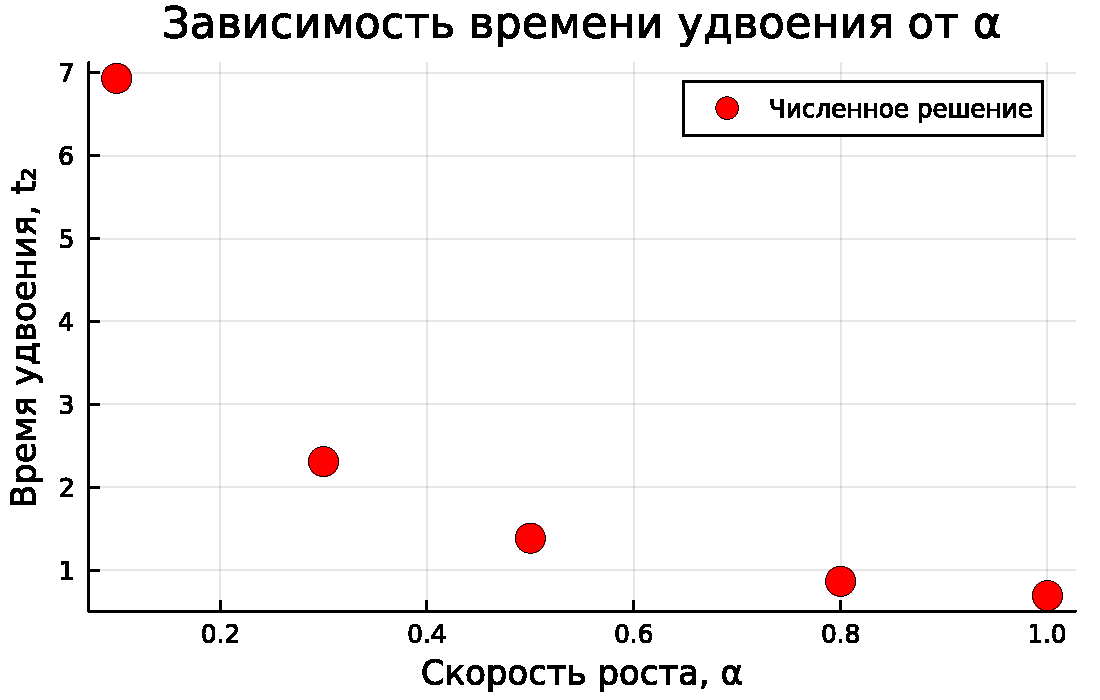
\includegraphics[keepaspectratio]{report_files/figure-pdf/cell-20-output-1.pdf}}

Теоретическая кривая: t₂ = ln(2) / α

\begin{Shaded}
\begin{Highlighting}[]
\NormalTok{α\_range }\OperatorTok{=} \FloatTok{0.1}\OperatorTok{:}\FloatTok{0.01}\OperatorTok{:}\FloatTok{1.0}

\FunctionTok{plot!}\NormalTok{(}
\NormalTok{    p3,}
\NormalTok{    α\_range,}
    \FunctionTok{log}\NormalTok{(}\FloatTok{2}\NormalTok{) }\OperatorTok{./}\NormalTok{ α\_range,}
\NormalTok{    label}\OperatorTok{=}\StringTok{"Теория: t₂ = ln(2)/α"}\NormalTok{,}
\NormalTok{    lw}\OperatorTok{=}\FloatTok{2}\NormalTok{,}
\NormalTok{    linestyle}\OperatorTok{=:}\NormalTok{dash,}
\NormalTok{    linecolor}\OperatorTok{=:}\NormalTok{blue}
\NormalTok{)}

\FunctionTok{savefig}\NormalTok{(}
    \FunctionTok{plotsdir}\NormalTok{(}
\NormalTok{        script\_name,}
        \StringTok{"doubling\_time\_vs\_alpha.png"}
\NormalTok{    )}
\NormalTok{)}
\end{Highlighting}
\end{Shaded}

\begin{verbatim}
"/home/kiran/work/study/2026-1/2026-1==study--mathmod/2026-1--study--mathmod/labs/lab01/project/plots/startup/doubling_time_vs_alpha.png"
\end{verbatim}

\section{Бенчмаркинг с разными
параметрами}\label{ux431ux435ux43dux447ux43cux430ux440ux43aux438ux43dux433-ux441-ux440ux430ux437ux43dux44bux43cux438-ux43fux430ux440ux430ux43cux435ux442ux440ux430ux43cux438}

\begin{Shaded}
\begin{Highlighting}[]
\FunctionTok{println}\NormalTok{(}\StringTok{"}\SpecialCharTok{\textbackslash{}n}\StringTok{"} \OperatorTok{*} \StringTok{"="}\OperatorTok{\^{}}\FloatTok{60}\NormalTok{)}
\FunctionTok{println}\NormalTok{(}\StringTok{"Бенчмаркинг для разных значений α"}\NormalTok{)}
\FunctionTok{println}\NormalTok{(}\StringTok{"="}\OperatorTok{\^{}}\FloatTok{60}\NormalTok{)}

\NormalTok{benchmark\_results }\OperatorTok{=}\NormalTok{ []}

\ControlFlowTok{for}\NormalTok{ α\_value }\KeywordTok{in}\NormalTok{ param\_grid[}\OperatorTok{:}\NormalTok{α]}

\NormalTok{    bench\_params }\OperatorTok{=} \FunctionTok{Dict}\NormalTok{(}
        \OperatorTok{:}\NormalTok{u0 }\OperatorTok{=\textgreater{}}\NormalTok{ [}\FloatTok{1.0}\NormalTok{],}
        \OperatorTok{:}\NormalTok{α }\OperatorTok{=\textgreater{}}\NormalTok{ α\_value,}
        \OperatorTok{:}\NormalTok{tspan }\OperatorTok{=\textgreater{}}\NormalTok{ (}\FloatTok{0.0}\NormalTok{, }\FloatTok{10.0}\NormalTok{),}
        \OperatorTok{:}\NormalTok{solver }\OperatorTok{=\textgreater{}} \FunctionTok{Tsit5}\NormalTok{(),}
        \OperatorTok{:}\NormalTok{saveat }\OperatorTok{=\textgreater{}} \FloatTok{0.1}
\NormalTok{    )}

    \KeywordTok{function} \FunctionTok{benchmark\_run}\NormalTok{()}

\NormalTok{        prob }\OperatorTok{=} \FunctionTok{ODEProblem}\NormalTok{(}
\NormalTok{            exponential\_growth!,}
\NormalTok{            bench\_params[}\OperatorTok{:}\NormalTok{u0],}
\NormalTok{            bench\_params[}\OperatorTok{:}\NormalTok{tspan],}
\NormalTok{            (α}\OperatorTok{=}\NormalTok{bench\_params[}\OperatorTok{:}\NormalTok{α],)}
\NormalTok{        )}

        \ControlFlowTok{return} \FunctionTok{solve}\NormalTok{(}
\NormalTok{            prob,}
\NormalTok{            bench\_params[}\OperatorTok{:}\NormalTok{solver];}
\NormalTok{            saveat}\OperatorTok{=}\NormalTok{bench\_params[}\OperatorTok{:}\NormalTok{saveat]}
\NormalTok{        )}
    \ControlFlowTok{end}

    \FunctionTok{println}\NormalTok{(}\StringTok{"}\SpecialCharTok{\textbackslash{}n}\StringTok{Бенчмарк для α = }\SpecialCharTok{$}\StringTok{α}\NormalTok{\_value}\StringTok{:"}\NormalTok{)}

\NormalTok{    b }\OperatorTok{=} \PreprocessorTok{@benchmark} \OperatorTok{$}\FunctionTok{benchmark\_run}\NormalTok{() samples}\OperatorTok{=}\FloatTok{100}\NormalTok{ evals}\OperatorTok{=}\FloatTok{1}

    \FunctionTok{push!}\NormalTok{(}
\NormalTok{        benchmark\_results,}
\NormalTok{        (}
\NormalTok{            α}\OperatorTok{=}\NormalTok{α\_value,}
\NormalTok{            time}\OperatorTok{=}\FunctionTok{median}\NormalTok{(b).time }\OperatorTok{/} \FloatTok{1e9}
\NormalTok{        )}
\NormalTok{    )}

    \FunctionTok{println}\NormalTok{(}
        \StringTok{" Среднее время: "}\NormalTok{,}
        \FunctionTok{round}\NormalTok{(}
            \FunctionTok{median}\NormalTok{(b).time }\OperatorTok{/} \FloatTok{1e9}\NormalTok{;}
\NormalTok{            digits}\OperatorTok{=}\FloatTok{4}
\NormalTok{        ),}
        \StringTok{" сек"}
\NormalTok{    )}
\KeywordTok{end}
\end{Highlighting}
\end{Shaded}

\begin{verbatim}

============================================================
Бенчмаркинг для разных значений α
============================================================

Бенчмарк для α = 0.1:
 Среднее время: 0.0001 сек

Бенчмарк для α = 0.3:
 Среднее время: 0.0001 сек

Бенчмарк для α = 0.5:
 Среднее время: 0.0001 сек

Бенчмарк для α = 0.8:
 Среднее время: 0.0001 сек

Бенчмарк для α = 1.0:
 Среднее время: 0.0001 сек
\end{verbatim}

\section{График времени
вычисления}\label{ux433ux440ux430ux444ux438ux43a-ux432ux440ux435ux43cux435ux43dux438-ux432ux44bux447ux438ux441ux43bux435ux43dux438ux44f}

\begin{Shaded}
\begin{Highlighting}[]
\NormalTok{bench\_df }\OperatorTok{=} \FunctionTok{DataFrame}\NormalTok{(benchmark\_results)}

\NormalTok{p4 }\OperatorTok{=} \FunctionTok{plot}\NormalTok{(}
\NormalTok{    bench\_df.α,}
\NormalTok{    bench\_df.time,}
\NormalTok{    seriestype}\OperatorTok{=:}\NormalTok{scatter,}
\NormalTok{    label}\OperatorTok{=}\StringTok{"Время вычисления"}\NormalTok{,}
\NormalTok{    xlabel}\OperatorTok{=}\StringTok{"Скорость роста, α"}\NormalTok{,}
\NormalTok{    ylabel}\OperatorTok{=}\StringTok{"Время вычисления, сек"}\NormalTok{,}
\NormalTok{    title}\OperatorTok{=}\StringTok{"Зависимость времени вычисления от α"}\NormalTok{,}
\NormalTok{    markersize}\OperatorTok{=}\FloatTok{8}\NormalTok{,}
\NormalTok{    markercolor}\OperatorTok{=:}\NormalTok{green,}
\NormalTok{    legend}\OperatorTok{=:}\NormalTok{topleft}
\NormalTok{)}

\FunctionTok{savefig}\NormalTok{(}
    \FunctionTok{plotsdir}\NormalTok{(}
\NormalTok{        script\_name,}
        \StringTok{"computation\_time\_vs\_alpha.png"}
\NormalTok{    )}
\NormalTok{)}
\end{Highlighting}
\end{Shaded}

\begin{verbatim}
"/home/kiran/work/study/2026-1/2026-1==study--mathmod/2026-1--study--mathmod/labs/lab01/project/plots/startup/computation_time_vs_alpha.png"
\end{verbatim}

\section{Сохранение всех
результатов}\label{ux441ux43eux445ux440ux430ux43dux435ux43dux438ux435-ux432ux441ux435ux445-ux440ux435ux437ux443ux43bux44cux442ux430ux442ux43eux432}

\begin{Shaded}
\begin{Highlighting}[]
\PreprocessorTok{@save} \FunctionTok{datadir}\NormalTok{(}
\NormalTok{    script\_name,}
    \StringTok{"all\_results.jld2"}
\NormalTok{) base\_params param\_grid all\_params results\_df bench\_df}

\PreprocessorTok{@save} \FunctionTok{datadir}\NormalTok{(}
\NormalTok{    script\_name,}
    \StringTok{"all\_plots.jld2"}
\NormalTok{) p1 p2 p3 p4}

\FunctionTok{println}\NormalTok{(}\StringTok{"}\SpecialCharTok{\textbackslash{}n}\StringTok{"} \OperatorTok{*} \StringTok{"="}\OperatorTok{\^{}}\FloatTok{60}\NormalTok{)}
\FunctionTok{println}\NormalTok{(}\StringTok{"ЛАБОРАТОРНАЯ РАБОТА ЗАВЕРШЕНА"}\NormalTok{)}
\FunctionTok{println}\NormalTok{(}\StringTok{"="}\OperatorTok{\^{}}\FloatTok{60}\NormalTok{)}

\FunctionTok{println}\NormalTok{(}\StringTok{"}\SpecialCharTok{\textbackslash{}n}\StringTok{Результаты сохранены в:"}\NormalTok{)}
\FunctionTok{println}\NormalTok{(}
    \StringTok{" • data/}\SpecialCharTok{$}\NormalTok{(script\_name)}\StringTok{/single/ {-} базовый эксперимент"}
\NormalTok{)}
\FunctionTok{println}\NormalTok{(}
    \StringTok{" • data/}\SpecialCharTok{$}\NormalTok{(script\_name)}\StringTok{/parametric\_scan/ {-} параметрическое сканирование"}
\NormalTok{)}
\FunctionTok{println}\NormalTok{(}
    \StringTok{" • data/}\SpecialCharTok{$}\NormalTok{(script\_name)}\StringTok{/all\_results.jld2 {-} сводные данные"}
\NormalTok{)}
\FunctionTok{println}\NormalTok{(}
    \StringTok{" • plots/}\SpecialCharTok{$}\NormalTok{(script\_name)}\StringTok{/ {-} все графики"}
\NormalTok{)}
\FunctionTok{println}\NormalTok{(}
    \StringTok{" • data/}\SpecialCharTok{$}\NormalTok{(script\_name)}\StringTok{/all\_plots.jld2 {-} объекты графиков"}
\NormalTok{)}

\FunctionTok{println}\NormalTok{(}\StringTok{"}\SpecialCharTok{\textbackslash{}n}\StringTok{Для анализа результатов используйте:"}\NormalTok{)}
\FunctionTok{println}\NormalTok{(}\StringTok{" using JLD2, DataFrames"}\NormalTok{)}
\FunctionTok{println}\NormalTok{(}
    \StringTok{" @load }\SpecialCharTok{\textbackslash{}"}\StringTok{data/}\SpecialCharTok{$}\NormalTok{(script\_name)}\StringTok{/all\_results.jld2}\SpecialCharTok{\textbackslash{}"}\StringTok{"}
\NormalTok{)}
\FunctionTok{println}\NormalTok{(}\StringTok{" println(results\_df)"}\NormalTok{)}
\end{Highlighting}
\end{Shaded}

\begin{verbatim}

============================================================
ЛАБОРАТОРНАЯ РАБОТА ЗАВЕРШЕНА
============================================================

Результаты сохранены в:
 • data/startup/single/ - базовый эксперимент
 • data/startup/parametric_scan/ - параметрическое сканирование
 • data/startup/all_results.jld2 - сводные данные
 • plots/startup/ - все графики
 • data/startup/all_plots.jld2 - объекты графиков

Для анализа результатов используйте:
 using JLD2, DataFrames
 @load "data/startup/all_results.jld2"
 println(results_df)
\end{verbatim}

\begin{figure}[H]

{\centering 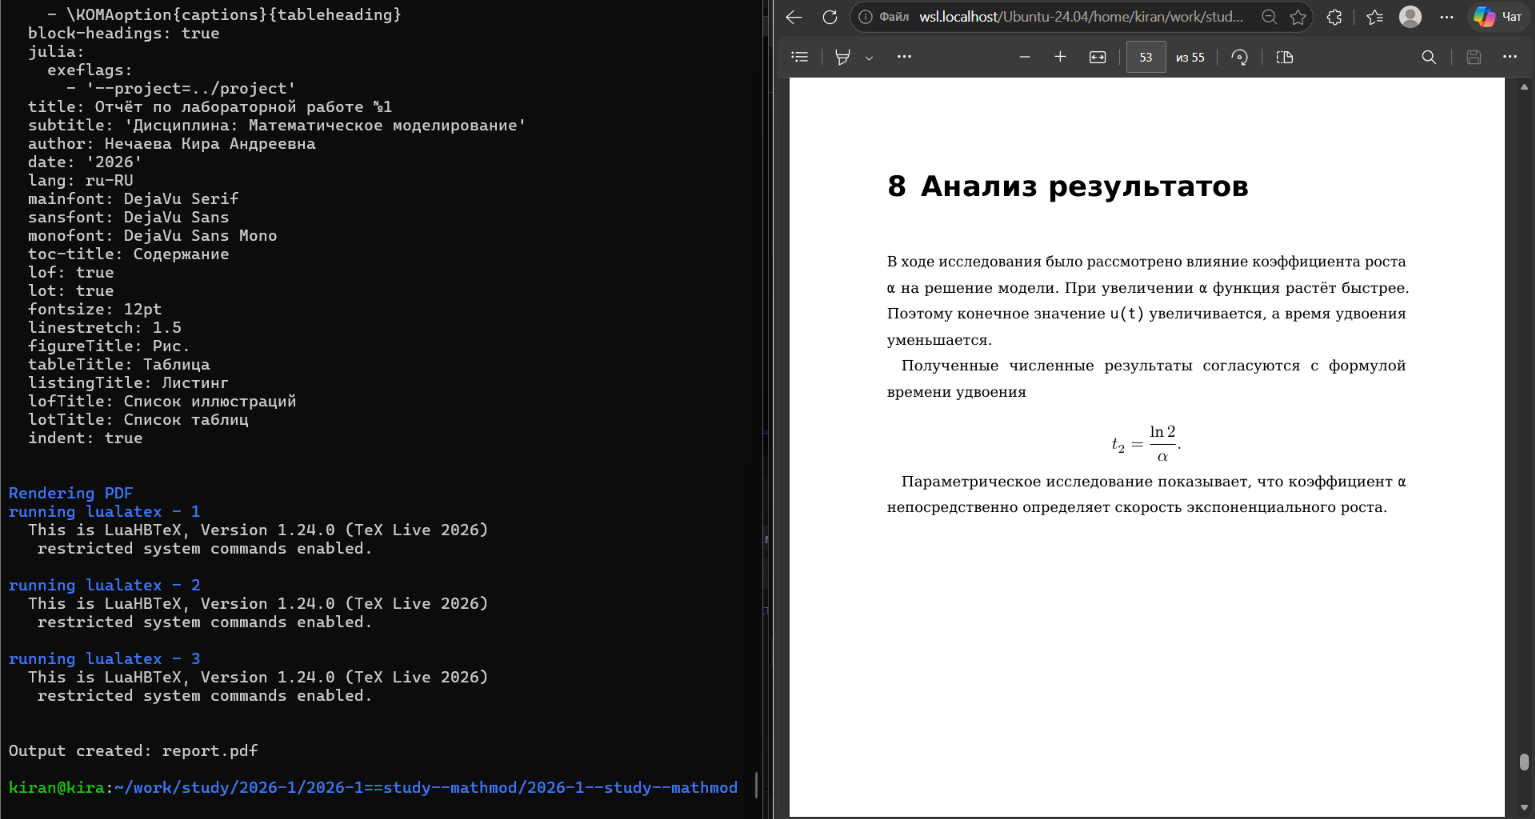
\includegraphics[width=0.7\linewidth,height=\textheight,keepaspectratio]{image/27.png}

}

\caption{Итоговая сборка отчёта}

\end{figure}%

\chapter{Анализ
результатов}\label{ux430ux43dux430ux43bux438ux437-ux440ux435ux437ux443ux43bux44cux442ux430ux442ux43eux432-1}

В ходе исследования было рассмотрено влияние коэффициента роста
\texttt{α} на решение модели. При увеличении \texttt{α} функция растёт
быстрее. Поэтому конечное значение \texttt{u(t)} увеличивается, а время
удвоения уменьшается.

Полученные численные результаты согласуются с формулой времени удвоения

\[
t_2 = \frac{\ln 2}{\alpha}.
\]

Параметрическое исследование показывает, что коэффициент \texttt{α}
непосредственно определяет скорость экспоненциального роста.

\chapter{Вывод}\label{ux432ux44bux432ux43eux434}

В ходе лабораторной работы было подготовлено рабочее пространство курса
и создан проект DrWatson. Были установлены необходимые пакеты Julia и
реализована модель экспоненциального роста.

Программа была преобразована в литературный стиль. Из литературного кода
были автоматически сгенерированы чистый код, Jupyter notebook и
документация Quarto.

Также было выполнено параметрическое исследование модели для нескольких
значений коэффициента роста. Результаты показали, что увеличение
\texttt{α} приводит к более быстрому росту функции и уменьшению времени
удвоения.

Сгенерированная документация для обеих версий программы была
интегрирована в отчёт.

\chapter*{Список
литературы}\label{ux441ux43fux438ux441ux43eux43a-ux43bux438ux442ux435ux440ux430ux442ux443ux440ux44b}
\addcontentsline{toc}{chapter}{Список литературы}

\begin{enumerate}
\def\labelenumi{\arabic{enumi}.}
\tightlist
\item
  Методические материалы к лабораторной работе №1 по математическому
  моделированию.
\end{enumerate}




\end{document}
